\documentclass[twoside]{book}

% Packages required by doxygen
\usepackage{fixltx2e}
\usepackage{calc}
\usepackage{doxygen}
\usepackage{graphicx}
\usepackage[utf8]{inputenc}
\usepackage{makeidx}
\usepackage{multicol}
\usepackage{multirow}
\PassOptionsToPackage{warn}{textcomp}
\usepackage{textcomp}
\usepackage[nointegrals]{wasysym}
\usepackage[table]{xcolor}

% Font selection
\usepackage[T1]{fontenc}
\usepackage{mathptmx}
\usepackage[scaled=.90]{helvet}
\usepackage{courier}
\usepackage{amssymb}
\usepackage{sectsty}
\renewcommand{\familydefault}{\sfdefault}
\allsectionsfont{%
  \fontseries{bc}\selectfont%
  \color{darkgray}%
}
\renewcommand{\DoxyLabelFont}{%
  \fontseries{bc}\selectfont%
  \color{darkgray}%
}
\newcommand{\+}{\discretionary{\mbox{\scriptsize$\hookleftarrow$}}{}{}}

% Page & text layout
\usepackage{geometry}
\geometry{%
  a4paper,%
  top=2.5cm,%
  bottom=2.5cm,%
  left=2.5cm,%
  right=2.5cm%
}
\tolerance=750
\hfuzz=15pt
\hbadness=750
\setlength{\emergencystretch}{15pt}
\setlength{\parindent}{0cm}
\setlength{\parskip}{0.2cm}
\makeatletter
\renewcommand{\paragraph}{%
  \@startsection{paragraph}{4}{0ex}{-1.0ex}{1.0ex}{%
    \normalfont\normalsize\bfseries\SS@parafont%
  }%
}
\renewcommand{\subparagraph}{%
  \@startsection{subparagraph}{5}{0ex}{-1.0ex}{1.0ex}{%
    \normalfont\normalsize\bfseries\SS@subparafont%
  }%
}
\makeatother

% Headers & footers
\usepackage{fancyhdr}
\pagestyle{fancyplain}
\fancyhead[LE]{\fancyplain{}{\bfseries\thepage}}
\fancyhead[CE]{\fancyplain{}{}}
\fancyhead[RE]{\fancyplain{}{\bfseries\leftmark}}
\fancyhead[LO]{\fancyplain{}{\bfseries\rightmark}}
\fancyhead[CO]{\fancyplain{}{}}
\fancyhead[RO]{\fancyplain{}{\bfseries\thepage}}
\fancyfoot[LE]{\fancyplain{}{}}
\fancyfoot[CE]{\fancyplain{}{}}
\fancyfoot[RE]{\fancyplain{}{\bfseries\scriptsize Generated on Wed Dec 10 2014 00\+:57\+:00 for Game Project by Doxygen }}
\fancyfoot[LO]{\fancyplain{}{\bfseries\scriptsize Generated on Wed Dec 10 2014 00\+:57\+:00 for Game Project by Doxygen }}
\fancyfoot[CO]{\fancyplain{}{}}
\fancyfoot[RO]{\fancyplain{}{}}
\renewcommand{\footrulewidth}{0.4pt}
\renewcommand{\chaptermark}[1]{%
  \markboth{#1}{}%
}
\renewcommand{\sectionmark}[1]{%
  \markright{\thesection\ #1}%
}

% Indices & bibliography
\usepackage{natbib}
\usepackage[titles]{tocloft}
\setcounter{tocdepth}{3}
\setcounter{secnumdepth}{5}
\makeindex

% Custom commands
\newcommand{\clearemptydoublepage}{%
  \newpage{\pagestyle{empty}\cleardoublepage}%
}


%===== C O N T E N T S =====

\begin{document}

% Titlepage & ToC
\pagenumbering{roman}
\begin{titlepage}
\vspace*{7cm}
\begin{center}%
{\Large Game Project }\\
\vspace*{1cm}
{\large Generated by Doxygen 1.8.8}\\
\vspace*{0.5cm}
{\small Wed Dec 10 2014 00:57:00}\\
\end{center}
\end{titlepage}
\clearemptydoublepage
\tableofcontents
\clearemptydoublepage
\pagenumbering{arabic}

%--- Begin generated contents ---
\chapter{Hierarchical Index}
\section{Class Hierarchy}
This inheritance list is sorted roughly, but not completely, alphabetically\+:\begin{DoxyCompactList}
\item \contentsline{section}{Pikachu}{\pageref{class_pikachu}}{}
\item Q\+Main\+Window\begin{DoxyCompactList}
\item \contentsline{section}{Main\+Window}{\pageref{class_main_window}}{}
\end{DoxyCompactList}
\item Q\+Widget\begin{DoxyCompactList}
\item \contentsline{section}{Game\+Board}{\pageref{class_game_board}}{}
\item \contentsline{section}{Game\+Over\+Widget}{\pageref{class_game_over_widget}}{}
\item \contentsline{section}{How\+To}{\pageref{class_how_to}}{}
\item \contentsline{section}{Quit\+Widget}{\pageref{class_quit_widget}}{}
\end{DoxyCompactList}
\end{DoxyCompactList}

\chapter{Class Index}
\section{Class List}
Here are the classes, structs, unions and interfaces with brief descriptions\+:\begin{DoxyCompactList}
\item\contentsline{section}{{\bf Game\+Board} \\*Displays the board on which the game is played~\newline
$\ast$ Top displays the lives and score~\newline
$\ast$$\ast$ lives stores pointers to Q\+Label objects displaying the images for each life~\newline
$\ast$ score\+\_\+label displays the score~\newline
 int score stores the score~\newline
$\ast$ Board displays the tiles~\newline
$\ast$$\ast$ labels stores pointers to Q\+Label objects displaying each tile~\newline
 board\+\_\+size stores the size of the board~\newline
 cursor\+\_\+location stores the location of the cursor~\newline
 life\+\_\+position stores the location of the extra life~\newline
 clicked stores whether the mouse was clicked~\newline
$\ast$ squirtle\+\_\+image stores the image of the squirtles~\newline
$\ast$ charmander\+\_\+image stores the image of the charmanders~\newline
$\ast$ attack\+\_\+image stores the image of the attack~\newline
 number\+\_\+squirtles stores the total number of squirtles on the board~\newline
 alive\+\_\+squirtles stores the number of squirtles that have yet to be defeated~\newline
 number\+\_\+charmanders stores the total number of charmanders on the board~\newline
 alive\+\_\+charmanders stores the number of charmanders that have yet to be defeated~\newline
$\ast$ q points to the \doxyref{Quit\+Widget}{p.}{class_quit_widget} object~\newline
$\ast$ m points to the \doxyref{Main\+Window}{p.}{class_main_window} object~\newline
$\ast$ g points to the \doxyref{Game\+Over\+Widget}{p.}{class_game_over_widget} object~\newline
$\ast$ pika points to the \doxyref{Pikachu}{p.}{class_pikachu} object controlled by the player }{\pageref{class_game_board}}{}
\item\contentsline{section}{{\bf Game\+Over\+Widget} \\*The \doxyref{Game\+Over\+Widget}{p.}{class_game_over_widget} class~\newline
$\ast$ over displays the \char`\"{}\+Game Over!\char`\"{} message~\newline
$\ast$ play\+Again takes the user to a new game~\newline
$\ast$ main\+Menu takes the user to the main menu~\newline
$\ast$ exit brings up the \doxyref{Quit\+Widget}{p.}{class_quit_widget}~\newline
$\ast$ mw points to the \doxyref{Main\+Window}{p.}{class_main_window}~\newline
$\ast$ board points to the \doxyref{Game\+Board}{p.}{class_game_board}~\newline
$\ast$ quit points to the \doxyref{Quit\+Widget}{p.}{class_quit_widget} }{\pageref{class_game_over_widget}}{}
\item\contentsline{section}{{\bf How\+To} \\*Displays controls for how the game is played~\newline
$\ast$ back closes \doxyref{How\+To}{p.}{class_how_to}, taking the user back to the \doxyref{Main\+Window}{p.}{class_main_window} }{\pageref{class_how_to}}{}
\item\contentsline{section}{{\bf Main\+Window} \\*Displays the main menu for the game~\newline
$\ast$ board points to the \doxyref{Game\+Board}{p.}{class_game_board}~\newline
$\ast$ how points to the \doxyref{How\+To}{p.}{class_how_to}~\newline
$\ast$ quit points to the \doxyref{Quit\+Widget}{p.}{class_quit_widget}~\newline
$\ast$ title displays the title of the game~\newline
$\ast$ play takes the user to the game board~\newline
$\ast$ howto takes the user to the \doxyref{How\+To}{p.}{class_how_to} screen~\newline
$\ast$ exit brings up the \doxyref{Quit\+Widget}{p.}{class_quit_widget}~\newline
$\ast$ buttons stores the layout for the Q\+Push\+Button objects~\newline
$\ast$ final\+\_\+layout stores the final layout~\newline
$\ast$ central is the central widget applying final\+\_\+layout }{\pageref{class_main_window}}{}
\item\contentsline{section}{{\bf Pikachu} \\*User controlled \doxyref{Pikachu}{p.}{class_pikachu}~\newline
 x, y store the coordinates~\newline
 int lives stores the number of lives~\newline
 int max\+\_\+lives stores the max number of lives~\newline
 int dir represents direction (0 = up, 1 = down, 2 = left, 3 = right)~\newline
$\ast$ up\+\_\+image stores the facing up image~\newline
$\ast$ down\+\_\+image stores the facing down image~\newline
$\ast$ left\+\_\+image stores the facing left image~\newline
$\ast$ right\+\_\+image stores the facing right image }{\pageref{class_pikachu}}{}
\item\contentsline{section}{{\bf Quit\+Widget} \\*Displays the confirmation message upon exit~\newline
$\ast$ ok closes the application when clicked~\newline
$\ast$ sure displays the confirmation message~\newline
$\ast$ cancel returns the user to the main menu }{\pageref{class_quit_widget}}{}
\end{DoxyCompactList}

\chapter{File Index}
\section{File List}
Here is a list of all files with brief descriptions\+:\begin{DoxyCompactList}
\item\contentsline{section}{Headers/{\bf gameboard.\+h} }{\pageref{gameboard_8h}}{}
\item\contentsline{section}{Headers/{\bf gameoverwidget.\+h} }{\pageref{gameoverwidget_8h}}{}
\item\contentsline{section}{Headers/{\bf howto.\+h} }{\pageref{howto_8h}}{}
\item\contentsline{section}{Headers/{\bf mainwindow.\+h} }{\pageref{mainwindow_8h}}{}
\item\contentsline{section}{Headers/{\bf pikachu.\+h} }{\pageref{pikachu_8h}}{}
\item\contentsline{section}{Headers/{\bf quitwidget.\+h} }{\pageref{quitwidget_8h}}{}
\item\contentsline{section}{Sources/{\bf gameboard.\+cpp} }{\pageref{gameboard_8cpp}}{}
\item\contentsline{section}{Sources/{\bf gameoverwidget.\+cpp} }{\pageref{gameoverwidget_8cpp}}{}
\item\contentsline{section}{Sources/{\bf howto.\+cpp} }{\pageref{howto_8cpp}}{}
\item\contentsline{section}{Sources/{\bf main.\+cpp} }{\pageref{main_8cpp}}{}
\item\contentsline{section}{Sources/{\bf mainwindow.\+cpp} }{\pageref{mainwindow_8cpp}}{}
\item\contentsline{section}{Sources/{\bf pikachu.\+cpp} }{\pageref{pikachu_8cpp}}{}
\item\contentsline{section}{Sources/{\bf quitwidget.\+cpp} }{\pageref{quitwidget_8cpp}}{}
\end{DoxyCompactList}

\chapter{Class Documentation}
\section{Game\+Board Class Reference}
\label{class_game_board}\index{Game\+Board@{Game\+Board}}


The \doxyref{Game\+Board}{p.}{class_game_board} class displays the board on which the game is played~\newline
$\ast$ Top displays the lives and score~\newline
$\ast$$\ast$ lives stores pointers to Q\+Label objects displaying the images for each life~\newline
$\ast$ score\+\_\+label displays the score~\newline
 int score stores the score~\newline
$\ast$ Board displays the tiles~\newline
$\ast$$\ast$ labels stores pointers to Q\+Label objects displaying each tile~\newline
 board\+\_\+size stores the size of the board~\newline
 cursor\+\_\+location stores the location of the cursor~\newline
 life\+\_\+position stores the location of the extra life~\newline
 clicked stores whether the mouse was clicked~\newline
$\ast$ squirtle\+\_\+image stores the image of the squirtles~\newline
$\ast$ charmander\+\_\+image stores the image of the charmanders~\newline
$\ast$ attack\+\_\+image stores the image of the attack~\newline
 number\+\_\+squirtles stores the total number of squirtles on the board~\newline
 alive\+\_\+squirtles stores the number of squirtles that have yet to be defeated~\newline
 number\+\_\+charmanders stores the total number of charmanders on the board~\newline
 alive\+\_\+charmanders stores the number of charmanders that have yet to be defeated~\newline
$\ast$ q points to the \doxyref{Quit\+Widget}{p.}{class_quit_widget} object~\newline
$\ast$ m points to the \doxyref{Main\+Window}{p.}{class_main_window} object~\newline
$\ast$ g points to the \doxyref{Game\+Over\+Widget}{p.}{class_game_over_widget} object~\newline
$\ast$ pika points to the \doxyref{Pikachu}{p.}{class_pikachu} object controlled by the player.  




{\ttfamily \#include $<$gameboard.\+h$>$}

Inheritance diagram for Game\+Board\+:\begin{figure}[H]
\begin{center}
\leavevmode
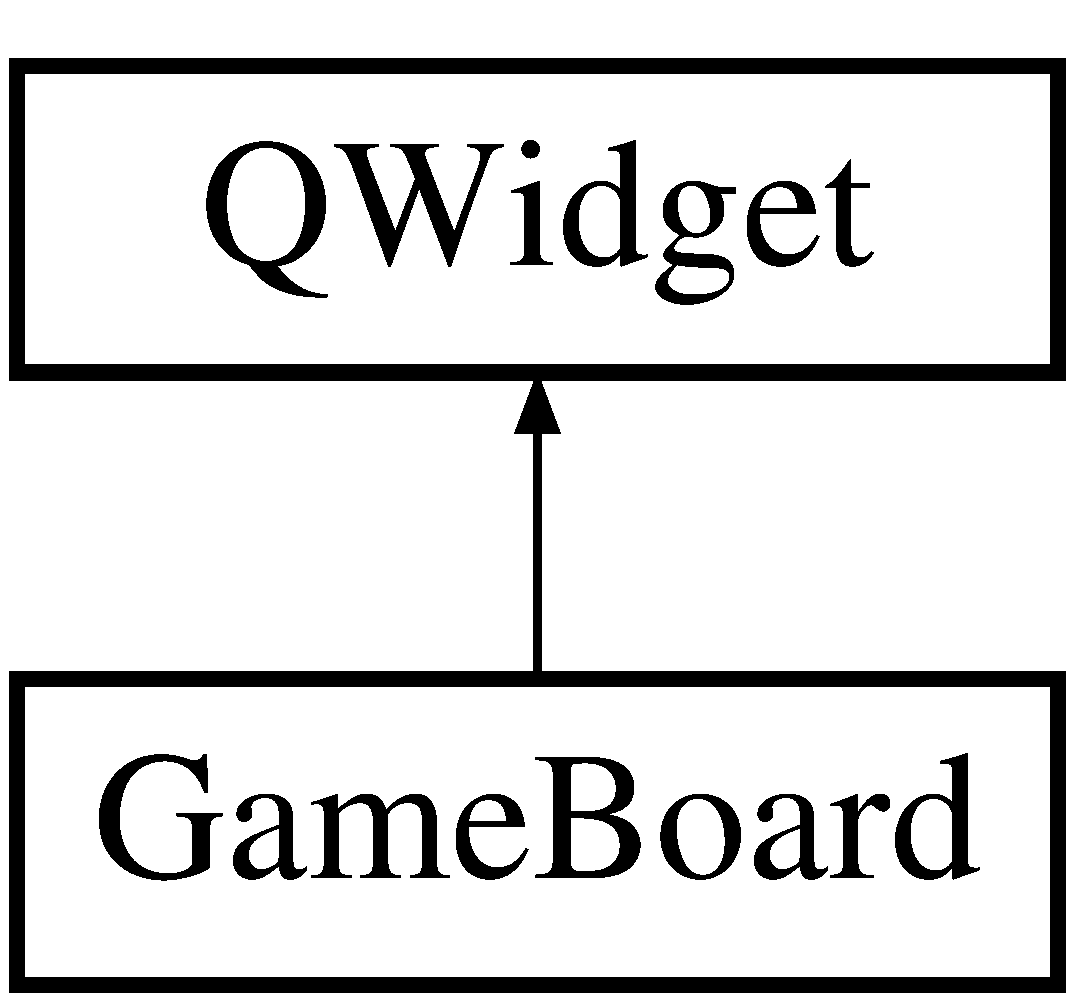
\includegraphics[height=2.000000cm]{class_game_board}
\end{center}
\end{figure}
\subsection*{Public Slots}
\begin{DoxyCompactItemize}
\item 
void {\bf update\+Squirtles} ()
\begin{DoxyCompactList}\small\item\em update\+Squirtles updates the squirtles on the board \end{DoxyCompactList}\item 
void {\bf update\+Charmanders} ()
\begin{DoxyCompactList}\small\item\em update\+Charmanders updates the charmanders on the board \end{DoxyCompactList}\item 
void {\bf display\+Life} ()
\begin{DoxyCompactList}\small\item\em display\+Life puts extra life on board if current lives $<$ max lives \end{DoxyCompactList}\item 
void {\bf clear\+Attack} ()
\begin{DoxyCompactList}\small\item\em clear\+Attack clears attack image \end{DoxyCompactList}\end{DoxyCompactItemize}
\subsection*{Signals}
\begin{DoxyCompactItemize}
\item 
void {\bf mouse\+Above} ()
\begin{DoxyCompactList}\small\item\em mouse\+Above emitted when mouse is above \doxyref{Pikachu}{p.}{class_pikachu} \end{DoxyCompactList}\item 
void {\bf mouse\+Below} ()
\begin{DoxyCompactList}\small\item\em mouse\+Below emitted when mouse is below \doxyref{Pikachu}{p.}{class_pikachu} \end{DoxyCompactList}\item 
void {\bf mouse\+To\+Left} ()
\begin{DoxyCompactList}\small\item\em mouse\+To\+Left emitted when mouse is left of \doxyref{Pikachu}{p.}{class_pikachu} \end{DoxyCompactList}\item 
void {\bf mouse\+To\+Right} ()
\begin{DoxyCompactList}\small\item\em mouse\+To\+Right emitted when mouse is right of \doxyref{Pikachu}{p.}{class_pikachu} \end{DoxyCompactList}\end{DoxyCompactItemize}
\subsection*{Public Member Functions}
\begin{DoxyCompactItemize}
\item 
{\bf Game\+Board} (Q\+Widget $\ast$parent=0)
\item 
{\bf $\sim$\+Game\+Board} ()
\item 
void {\bf key\+Press\+Event} (Q\+Key\+Event $\ast$event)
\begin{DoxyCompactList}\small\item\em key\+Press\+Event determines what happens when the keyboard is pressed \end{DoxyCompactList}\item 
void {\bf paint\+Event} (Q\+Paint\+Event $\ast$e)
\begin{DoxyCompactList}\small\item\em paint\+Event repaints the game \end{DoxyCompactList}\item 
void {\bf close\+Event} (Q\+Close\+Event $\ast$e)
\begin{DoxyCompactList}\small\item\em close\+Event returns user to main menu when attempting to close \end{DoxyCompactList}\item 
void {\bf set\+Quit\+Widget} ({\bf Quit\+Widget} $\ast$quit\+\_\+widget)
\begin{DoxyCompactList}\small\item\em set\+Quit\+Widget sets \doxyref{Quit\+Widget}{p.}{class_quit_widget} \end{DoxyCompactList}\item 
void {\bf set\+Main\+Window} ({\bf Main\+Window} $\ast$main\+\_\+window)
\begin{DoxyCompactList}\small\item\em set\+Main\+Window sets \doxyref{Main\+Window}{p.}{class_main_window} \end{DoxyCompactList}\item 
void {\bf set\+Game\+Over\+Widget} ({\bf Game\+Over\+Widget} $\ast$game\+\_\+over)
\begin{DoxyCompactList}\small\item\em set\+Game\+Over\+Widget sets \doxyref{Game\+Over\+Widget}{p.}{class_game_over_widget} \end{DoxyCompactList}\item 
bool {\bf squirtle\+Available} ()
\begin{DoxyCompactList}\small\item\em squirtle\+Available determines if a squirtle is available for spawning \end{DoxyCompactList}\item 
bool {\bf charmander\+Available} ()
\begin{DoxyCompactList}\small\item\em charmander\+Available determines if a charmander is available for spawning \end{DoxyCompactList}\item 
bool {\bf position\+Available\+For\+Spawn} (int x, int y)
\begin{DoxyCompactList}\small\item\em position\+Available\+For\+Spawn determines if a squirtle can be spawned at target location \end{DoxyCompactList}\item 
bool {\bf valid\+Enemy\+Move} (int x, int y)
\begin{DoxyCompactList}\small\item\em valid\+Enemy\+Move \end{DoxyCompactList}\item 
bool {\bf defeated} ()
\begin{DoxyCompactList}\small\item\em defeated determines if \doxyref{Pikachu}{p.}{class_pikachu} is defeated \end{DoxyCompactList}\item 
bool {\bf game\+Over} ()
\begin{DoxyCompactList}\small\item\em game\+Over determines if the player loses \end{DoxyCompactList}\end{DoxyCompactItemize}


\subsection{Detailed Description}
The \doxyref{Game\+Board}{p.}{class_game_board} class displays the board on which the game is played~\newline
$\ast$ Top displays the lives and score~\newline
$\ast$$\ast$ lives stores pointers to Q\+Label objects displaying the images for each life~\newline
$\ast$ score\+\_\+label displays the score~\newline
 int score stores the score~\newline
$\ast$ Board displays the tiles~\newline
$\ast$$\ast$ labels stores pointers to Q\+Label objects displaying each tile~\newline
 board\+\_\+size stores the size of the board~\newline
 cursor\+\_\+location stores the location of the cursor~\newline
 life\+\_\+position stores the location of the extra life~\newline
 clicked stores whether the mouse was clicked~\newline
$\ast$ squirtle\+\_\+image stores the image of the squirtles~\newline
$\ast$ charmander\+\_\+image stores the image of the charmanders~\newline
$\ast$ attack\+\_\+image stores the image of the attack~\newline
 number\+\_\+squirtles stores the total number of squirtles on the board~\newline
 alive\+\_\+squirtles stores the number of squirtles that have yet to be defeated~\newline
 number\+\_\+charmanders stores the total number of charmanders on the board~\newline
 alive\+\_\+charmanders stores the number of charmanders that have yet to be defeated~\newline
$\ast$ q points to the \doxyref{Quit\+Widget}{p.}{class_quit_widget} object~\newline
$\ast$ m points to the \doxyref{Main\+Window}{p.}{class_main_window} object~\newline
$\ast$ g points to the \doxyref{Game\+Over\+Widget}{p.}{class_game_over_widget} object~\newline
$\ast$ pika points to the \doxyref{Pikachu}{p.}{class_pikachu} object controlled by the player. 

\subsection{Constructor \& Destructor Documentation}
\index{Game\+Board@{Game\+Board}!Game\+Board@{Game\+Board}}
\index{Game\+Board@{Game\+Board}!Game\+Board@{Game\+Board}}
\subsubsection[{Game\+Board}]{\setlength{\rightskip}{0pt plus 5cm}Game\+Board\+::\+Game\+Board (
\begin{DoxyParamCaption}
\item[{Q\+Widget $\ast$}]{parent = {\ttfamily 0}}
\end{DoxyParamCaption}
)\hspace{0.3cm}{\ttfamily [explicit]}}\label{class_game_board_ae4207b84e556e0794a4df666fb9a6463}
\index{Game\+Board@{Game\+Board}!````~Game\+Board@{$\sim$\+Game\+Board}}
\index{````~Game\+Board@{$\sim$\+Game\+Board}!Game\+Board@{Game\+Board}}
\subsubsection[{$\sim$\+Game\+Board}]{\setlength{\rightskip}{0pt plus 5cm}Game\+Board\+::$\sim$\+Game\+Board (
\begin{DoxyParamCaption}
{}
\end{DoxyParamCaption}
)}\label{class_game_board_a48e19b4953c87cc5eea1f9152d09499e}


\subsection{Member Function Documentation}
\index{Game\+Board@{Game\+Board}!charmander\+Available@{charmander\+Available}}
\index{charmander\+Available@{charmander\+Available}!Game\+Board@{Game\+Board}}
\subsubsection[{charmander\+Available}]{\setlength{\rightskip}{0pt plus 5cm}bool Game\+Board\+::charmander\+Available (
\begin{DoxyParamCaption}
{}
\end{DoxyParamCaption}
)}\label{class_game_board_a19d871e6b827f07449612f2963f42568}


charmander\+Available determines if a charmander is available for spawning 

\begin{DoxyReturn}{Returns}
true if a charmander if available 
\end{DoxyReturn}
\index{Game\+Board@{Game\+Board}!clear\+Attack@{clear\+Attack}}
\index{clear\+Attack@{clear\+Attack}!Game\+Board@{Game\+Board}}
\subsubsection[{clear\+Attack}]{\setlength{\rightskip}{0pt plus 5cm}void Game\+Board\+::clear\+Attack (
\begin{DoxyParamCaption}
{}
\end{DoxyParamCaption}
)\hspace{0.3cm}{\ttfamily [slot]}}\label{class_game_board_a99891f52fdfec6980fb87ef9e6f5ad6b}


clear\+Attack clears attack image 

\index{Game\+Board@{Game\+Board}!close\+Event@{close\+Event}}
\index{close\+Event@{close\+Event}!Game\+Board@{Game\+Board}}
\subsubsection[{close\+Event}]{\setlength{\rightskip}{0pt plus 5cm}void Game\+Board\+::close\+Event (
\begin{DoxyParamCaption}
\item[{Q\+Close\+Event $\ast$}]{e}
\end{DoxyParamCaption}
)}\label{class_game_board_a02f221bcf42b16b26af7920e5a65f3d2}


close\+Event returns user to main menu when attempting to close 


\begin{DoxyParams}{Parameters}
{\em e} & unused \\
\hline
\end{DoxyParams}
\index{Game\+Board@{Game\+Board}!defeated@{defeated}}
\index{defeated@{defeated}!Game\+Board@{Game\+Board}}
\subsubsection[{defeated}]{\setlength{\rightskip}{0pt plus 5cm}bool Game\+Board\+::defeated (
\begin{DoxyParamCaption}
{}
\end{DoxyParamCaption}
)}\label{class_game_board_aa6a94f182e06bef4894d0fa38d86ea83}


defeated determines if \doxyref{Pikachu}{p.}{class_pikachu} is defeated 

\begin{DoxyReturn}{Returns}
true if \doxyref{Pikachu}{p.}{class_pikachu} shares space with an enemy 
\end{DoxyReturn}
\index{Game\+Board@{Game\+Board}!display\+Life@{display\+Life}}
\index{display\+Life@{display\+Life}!Game\+Board@{Game\+Board}}
\subsubsection[{display\+Life}]{\setlength{\rightskip}{0pt plus 5cm}void Game\+Board\+::display\+Life (
\begin{DoxyParamCaption}
{}
\end{DoxyParamCaption}
)\hspace{0.3cm}{\ttfamily [slot]}}\label{class_game_board_a6549e8980a4a323d22b09fc19dd5313e}


display\+Life puts extra life on board if current lives $<$ max lives 

\index{Game\+Board@{Game\+Board}!game\+Over@{game\+Over}}
\index{game\+Over@{game\+Over}!Game\+Board@{Game\+Board}}
\subsubsection[{game\+Over}]{\setlength{\rightskip}{0pt plus 5cm}bool Game\+Board\+::game\+Over (
\begin{DoxyParamCaption}
{}
\end{DoxyParamCaption}
)}\label{class_game_board_aafda2038309024f8a7aa6607c68441e4}


game\+Over determines if the player loses 

\begin{DoxyReturn}{Returns}
true if all lives are gone 
\end{DoxyReturn}
\index{Game\+Board@{Game\+Board}!key\+Press\+Event@{key\+Press\+Event}}
\index{key\+Press\+Event@{key\+Press\+Event}!Game\+Board@{Game\+Board}}
\subsubsection[{key\+Press\+Event}]{\setlength{\rightskip}{0pt plus 5cm}void Game\+Board\+::key\+Press\+Event (
\begin{DoxyParamCaption}
\item[{Q\+Key\+Event $\ast$}]{event}
\end{DoxyParamCaption}
)}\label{class_game_board_a3fdf1e6bfcc24a0930196be5fc3150c1}


key\+Press\+Event determines what happens when the keyboard is pressed 


\begin{DoxyParams}{Parameters}
{\em event} & is the default event that occurs when the keyboard is pressed \\
\hline
\end{DoxyParams}
\index{Game\+Board@{Game\+Board}!mouse\+Above@{mouse\+Above}}
\index{mouse\+Above@{mouse\+Above}!Game\+Board@{Game\+Board}}
\subsubsection[{mouse\+Above}]{\setlength{\rightskip}{0pt plus 5cm}void Game\+Board\+::mouse\+Above (
\begin{DoxyParamCaption}
{}
\end{DoxyParamCaption}
)\hspace{0.3cm}{\ttfamily [signal]}}\label{class_game_board_acab5c422b54d51e2872619ea1ca6d231}


mouse\+Above emitted when mouse is above \doxyref{Pikachu}{p.}{class_pikachu} 

\index{Game\+Board@{Game\+Board}!mouse\+Below@{mouse\+Below}}
\index{mouse\+Below@{mouse\+Below}!Game\+Board@{Game\+Board}}
\subsubsection[{mouse\+Below}]{\setlength{\rightskip}{0pt plus 5cm}void Game\+Board\+::mouse\+Below (
\begin{DoxyParamCaption}
{}
\end{DoxyParamCaption}
)\hspace{0.3cm}{\ttfamily [signal]}}\label{class_game_board_a576cdef69a8b6bf38c4a689ec5ead7b0}


mouse\+Below emitted when mouse is below \doxyref{Pikachu}{p.}{class_pikachu} 

\index{Game\+Board@{Game\+Board}!mouse\+To\+Left@{mouse\+To\+Left}}
\index{mouse\+To\+Left@{mouse\+To\+Left}!Game\+Board@{Game\+Board}}
\subsubsection[{mouse\+To\+Left}]{\setlength{\rightskip}{0pt plus 5cm}void Game\+Board\+::mouse\+To\+Left (
\begin{DoxyParamCaption}
{}
\end{DoxyParamCaption}
)\hspace{0.3cm}{\ttfamily [signal]}}\label{class_game_board_af6017e753946ba9f846ac6f98fbb4162}


mouse\+To\+Left emitted when mouse is left of \doxyref{Pikachu}{p.}{class_pikachu} 

\index{Game\+Board@{Game\+Board}!mouse\+To\+Right@{mouse\+To\+Right}}
\index{mouse\+To\+Right@{mouse\+To\+Right}!Game\+Board@{Game\+Board}}
\subsubsection[{mouse\+To\+Right}]{\setlength{\rightskip}{0pt plus 5cm}void Game\+Board\+::mouse\+To\+Right (
\begin{DoxyParamCaption}
{}
\end{DoxyParamCaption}
)\hspace{0.3cm}{\ttfamily [signal]}}\label{class_game_board_acaade177399b644dfd954944711b94cb}


mouse\+To\+Right emitted when mouse is right of \doxyref{Pikachu}{p.}{class_pikachu} 

\index{Game\+Board@{Game\+Board}!paint\+Event@{paint\+Event}}
\index{paint\+Event@{paint\+Event}!Game\+Board@{Game\+Board}}
\subsubsection[{paint\+Event}]{\setlength{\rightskip}{0pt plus 5cm}void Game\+Board\+::paint\+Event (
\begin{DoxyParamCaption}
\item[{Q\+Paint\+Event $\ast$}]{e}
\end{DoxyParamCaption}
)}\label{class_game_board_a07896dc68fa3dc7ab7206e20da4c8dea}


paint\+Event repaints the game 


\begin{DoxyParams}{Parameters}
{\em e} & unused \\
\hline
\end{DoxyParams}
\index{Game\+Board@{Game\+Board}!position\+Available\+For\+Spawn@{position\+Available\+For\+Spawn}}
\index{position\+Available\+For\+Spawn@{position\+Available\+For\+Spawn}!Game\+Board@{Game\+Board}}
\subsubsection[{position\+Available\+For\+Spawn}]{\setlength{\rightskip}{0pt plus 5cm}bool Game\+Board\+::position\+Available\+For\+Spawn (
\begin{DoxyParamCaption}
\item[{int}]{x, }
\item[{int}]{y}
\end{DoxyParamCaption}
)}\label{class_game_board_adf3eae40924bfb011eae2d2a2585cd0e}


position\+Available\+For\+Spawn determines if a squirtle can be spawned at target location 


\begin{DoxyParams}{Parameters}
{\em x} & the target x value \\
\hline
{\em y} & the target y value \\
\hline
\end{DoxyParams}
\begin{DoxyReturn}{Returns}
true if space is unoccupied 
\end{DoxyReturn}
\index{Game\+Board@{Game\+Board}!set\+Game\+Over\+Widget@{set\+Game\+Over\+Widget}}
\index{set\+Game\+Over\+Widget@{set\+Game\+Over\+Widget}!Game\+Board@{Game\+Board}}
\subsubsection[{set\+Game\+Over\+Widget}]{\setlength{\rightskip}{0pt plus 5cm}void Game\+Board\+::set\+Game\+Over\+Widget (
\begin{DoxyParamCaption}
\item[{{\bf Game\+Over\+Widget} $\ast$}]{game\+\_\+over}
\end{DoxyParamCaption}
)}\label{class_game_board_a8143e2f240973110a4543008a89aff02}


set\+Game\+Over\+Widget sets \doxyref{Game\+Over\+Widget}{p.}{class_game_over_widget} 


\begin{DoxyParams}{Parameters}
{\em game\+\_\+over} & the \doxyref{Game\+Over\+Widget}{p.}{class_game_over_widget} input \\
\hline
\end{DoxyParams}
\index{Game\+Board@{Game\+Board}!set\+Main\+Window@{set\+Main\+Window}}
\index{set\+Main\+Window@{set\+Main\+Window}!Game\+Board@{Game\+Board}}
\subsubsection[{set\+Main\+Window}]{\setlength{\rightskip}{0pt plus 5cm}void Game\+Board\+::set\+Main\+Window (
\begin{DoxyParamCaption}
\item[{{\bf Main\+Window} $\ast$}]{main\+\_\+window}
\end{DoxyParamCaption}
)}\label{class_game_board_a36b37036f29a3805cd7fbcf8a51517f6}


set\+Main\+Window sets \doxyref{Main\+Window}{p.}{class_main_window} 


\begin{DoxyParams}{Parameters}
{\em main\+\_\+window} & the \doxyref{Main\+Window}{p.}{class_main_window} input \\
\hline
\end{DoxyParams}
\index{Game\+Board@{Game\+Board}!set\+Quit\+Widget@{set\+Quit\+Widget}}
\index{set\+Quit\+Widget@{set\+Quit\+Widget}!Game\+Board@{Game\+Board}}
\subsubsection[{set\+Quit\+Widget}]{\setlength{\rightskip}{0pt plus 5cm}void Game\+Board\+::set\+Quit\+Widget (
\begin{DoxyParamCaption}
\item[{{\bf Quit\+Widget} $\ast$}]{quit\+\_\+widget}
\end{DoxyParamCaption}
)}\label{class_game_board_a2c49afbf813d86425feb3b3ec71515ab}


set\+Quit\+Widget sets \doxyref{Quit\+Widget}{p.}{class_quit_widget} 


\begin{DoxyParams}{Parameters}
{\em quit\+\_\+widget} & the \doxyref{Quit\+Widget}{p.}{class_quit_widget} input \\
\hline
\end{DoxyParams}
\index{Game\+Board@{Game\+Board}!squirtle\+Available@{squirtle\+Available}}
\index{squirtle\+Available@{squirtle\+Available}!Game\+Board@{Game\+Board}}
\subsubsection[{squirtle\+Available}]{\setlength{\rightskip}{0pt plus 5cm}bool Game\+Board\+::squirtle\+Available (
\begin{DoxyParamCaption}
{}
\end{DoxyParamCaption}
)}\label{class_game_board_a0157acd6e868a25b86cc357a2d286d85}


squirtle\+Available determines if a squirtle is available for spawning 

\begin{DoxyReturn}{Returns}
true if a squirtle is available 
\end{DoxyReturn}
\index{Game\+Board@{Game\+Board}!update\+Charmanders@{update\+Charmanders}}
\index{update\+Charmanders@{update\+Charmanders}!Game\+Board@{Game\+Board}}
\subsubsection[{update\+Charmanders}]{\setlength{\rightskip}{0pt plus 5cm}void Game\+Board\+::update\+Charmanders (
\begin{DoxyParamCaption}
{}
\end{DoxyParamCaption}
)\hspace{0.3cm}{\ttfamily [slot]}}\label{class_game_board_a4db6ca244ab4a37e945256746681f518}


update\+Charmanders updates the charmanders on the board 

\index{Game\+Board@{Game\+Board}!update\+Squirtles@{update\+Squirtles}}
\index{update\+Squirtles@{update\+Squirtles}!Game\+Board@{Game\+Board}}
\subsubsection[{update\+Squirtles}]{\setlength{\rightskip}{0pt plus 5cm}void Game\+Board\+::update\+Squirtles (
\begin{DoxyParamCaption}
{}
\end{DoxyParamCaption}
)\hspace{0.3cm}{\ttfamily [slot]}}\label{class_game_board_a95649180cafe01439d27930b6f477c6d}


update\+Squirtles updates the squirtles on the board 

A\+T\+T\+E\+M\+P\+T A\+T T\+R\+Y\+I\+N\+G T\+O M\+A\+K\+E E\+N\+E\+M\+I\+E\+S S\+T\+O\+P F\+L\+A\+S\+H\+I\+N\+G std\+::uniform\+\_\+int\+\_\+distribution$<$int$>$ left\+\_\+or\+\_\+right(0, 1); std\+::vector$<$int$>$ px, py; for(size\+\_\+t i = 0; i $<$ number\+\_\+squirtles; i++) \{ px[i] = squirtle\+\_\+positions[i].rx(); py[i] = squirtle\+\_\+positions[i].ry();

int nx = px[i]; if (left\+\_\+or\+\_\+right(generator) == 0) nx--; else nx++;

don't move if move is not valid if(valid\+Enemy\+Move(nx, py[i])) squirtle\+\_\+positions[i].set\+X(nx); \}

Q\+Core\+Application\+::process\+Events(); repaint();

for(size\+\_\+t i = 0; i $<$ number\+\_\+squirtles; i++) \{ if(px[i] $>$= 0 \&\& py[i] $>$= 0 \&\& px[i] $<$ board\+\_\+size \&\& py[i] $<$ board\+\_\+size) labels[py[i] $\ast$ board\+\_\+size + px[i]]-\/$>$clear(); \}\index{Game\+Board@{Game\+Board}!valid\+Enemy\+Move@{valid\+Enemy\+Move}}
\index{valid\+Enemy\+Move@{valid\+Enemy\+Move}!Game\+Board@{Game\+Board}}
\subsubsection[{valid\+Enemy\+Move}]{\setlength{\rightskip}{0pt plus 5cm}bool Game\+Board\+::valid\+Enemy\+Move (
\begin{DoxyParamCaption}
\item[{int}]{x, }
\item[{int}]{y}
\end{DoxyParamCaption}
)}\label{class_game_board_a0584370f929ad836bd9d573fb7efee0c}


valid\+Enemy\+Move 


\begin{DoxyParams}{Parameters}
{\em x} & the target x value \\
\hline
{\em y} & the target y value \\
\hline
\end{DoxyParams}
\begin{DoxyReturn}{Returns}
true if space is unoccupied 
\end{DoxyReturn}


The documentation for this class was generated from the following files\+:\begin{DoxyCompactItemize}
\item 
Headers/{\bf gameboard.\+h}\item 
Sources/{\bf gameboard.\+cpp}\end{DoxyCompactItemize}

\section{Game\+Over\+Widget Class Reference}
\label{class_game_over_widget}\index{Game\+Over\+Widget@{Game\+Over\+Widget}}


The \doxyref{Game\+Over\+Widget}{p.}{class_game_over_widget} class~\newline
$\ast$ over displays the \char`\"{}\+Game Over!\char`\"{} message~\newline
$\ast$ play\+Again takes the user to a new game~\newline
$\ast$ main\+Menu takes the user to the main menu~\newline
$\ast$ exit brings up the \doxyref{Quit\+Widget}{p.}{class_quit_widget}~\newline
$\ast$ mw points to the \doxyref{Main\+Window}{p.}{class_main_window}~\newline
$\ast$ board points to the \doxyref{Game\+Board}{p.}{class_game_board}~\newline
$\ast$ quit points to the \doxyref{Quit\+Widget}{p.}{class_quit_widget}.  




{\ttfamily \#include $<$gameoverwidget.\+h$>$}

Inheritance diagram for Game\+Over\+Widget\+:\begin{figure}[H]
\begin{center}
\leavevmode
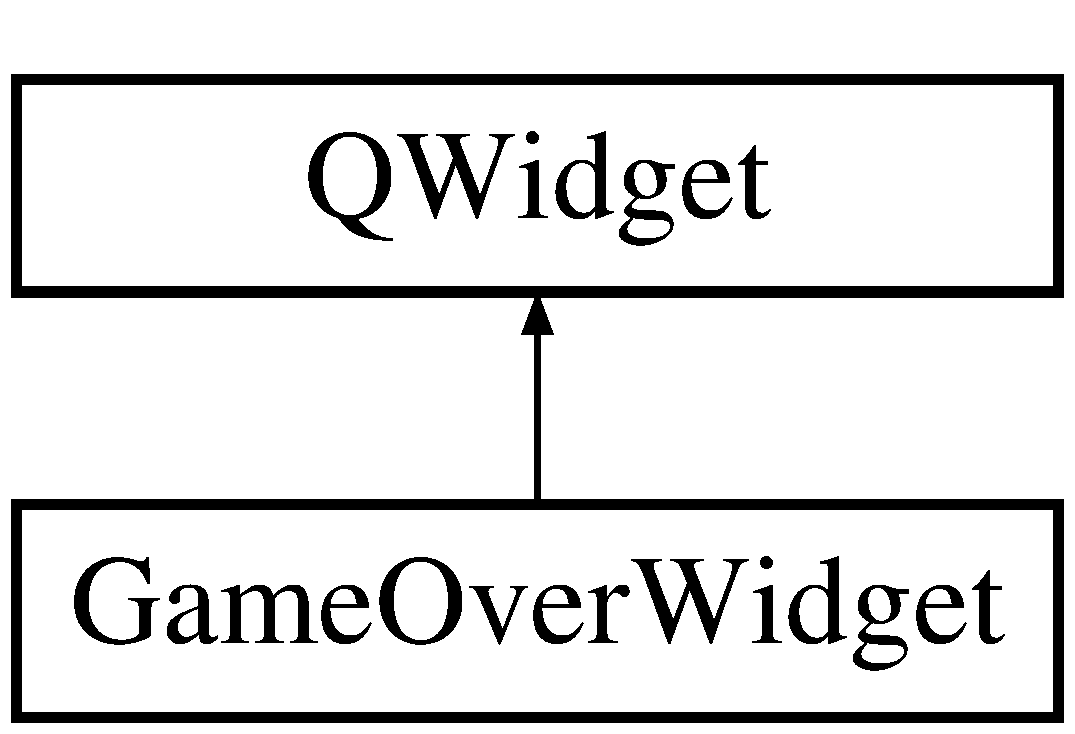
\includegraphics[height=2.000000cm]{class_game_over_widget}
\end{center}
\end{figure}
\subsection*{Public Slots}
\begin{DoxyCompactItemize}
\item 
void {\bf make\+Game\+Board} ()
\begin{DoxyCompactList}\small\item\em make\+Game\+Board makes a new \doxyref{Game\+Board}{p.}{class_game_board} \end{DoxyCompactList}\item 
void {\bf go\+To\+Menu} ()
\begin{DoxyCompactList}\small\item\em go\+To\+Menu takes the user to the main menu \end{DoxyCompactList}\end{DoxyCompactItemize}
\subsection*{Public Member Functions}
\begin{DoxyCompactItemize}
\item 
{\bf Game\+Over\+Widget} (Q\+Widget $\ast$parent=0)
\item 
{\bf $\sim$\+Game\+Over\+Widget} ()
\item 
void {\bf close\+Event} (Q\+Close\+Event $\ast$e)
\begin{DoxyCompactList}\small\item\em close\+Event opens the \doxyref{Quit\+Widget}{p.}{class_quit_widget} \end{DoxyCompactList}\item 
void {\bf set\+Main\+Window} ({\bf Main\+Window} $\ast$main\+\_\+window)
\begin{DoxyCompactList}\small\item\em set\+Main\+Window sets \doxyref{Main\+Window}{p.}{class_main_window} \end{DoxyCompactList}\item 
void {\bf set\+Game\+Board} ({\bf Game\+Board} $\ast$game\+\_\+board)
\begin{DoxyCompactList}\small\item\em set\+Game\+Board sets \doxyref{Game\+Board}{p.}{class_game_board} \end{DoxyCompactList}\item 
void {\bf set\+Quit\+Widget} ({\bf Quit\+Widget} $\ast$quit\+\_\+widget)
\begin{DoxyCompactList}\small\item\em set\+Quit\+Widget sets \doxyref{Quit\+Widget}{p.}{class_quit_widget} \end{DoxyCompactList}\end{DoxyCompactItemize}


\subsection{Detailed Description}
The \doxyref{Game\+Over\+Widget}{p.}{class_game_over_widget} class~\newline
$\ast$ over displays the \char`\"{}\+Game Over!\char`\"{} message~\newline
$\ast$ play\+Again takes the user to a new game~\newline
$\ast$ main\+Menu takes the user to the main menu~\newline
$\ast$ exit brings up the \doxyref{Quit\+Widget}{p.}{class_quit_widget}~\newline
$\ast$ mw points to the \doxyref{Main\+Window}{p.}{class_main_window}~\newline
$\ast$ board points to the \doxyref{Game\+Board}{p.}{class_game_board}~\newline
$\ast$ quit points to the \doxyref{Quit\+Widget}{p.}{class_quit_widget}. 

\subsection{Constructor \& Destructor Documentation}
\index{Game\+Over\+Widget@{Game\+Over\+Widget}!Game\+Over\+Widget@{Game\+Over\+Widget}}
\index{Game\+Over\+Widget@{Game\+Over\+Widget}!Game\+Over\+Widget@{Game\+Over\+Widget}}
\subsubsection[{Game\+Over\+Widget}]{\setlength{\rightskip}{0pt plus 5cm}Game\+Over\+Widget\+::\+Game\+Over\+Widget (
\begin{DoxyParamCaption}
\item[{Q\+Widget $\ast$}]{parent = {\ttfamily 0}}
\end{DoxyParamCaption}
)\hspace{0.3cm}{\ttfamily [explicit]}}\label{class_game_over_widget_a55d503250450c2b01e524fe3b976b083}
\index{Game\+Over\+Widget@{Game\+Over\+Widget}!````~Game\+Over\+Widget@{$\sim$\+Game\+Over\+Widget}}
\index{````~Game\+Over\+Widget@{$\sim$\+Game\+Over\+Widget}!Game\+Over\+Widget@{Game\+Over\+Widget}}
\subsubsection[{$\sim$\+Game\+Over\+Widget}]{\setlength{\rightskip}{0pt plus 5cm}Game\+Over\+Widget\+::$\sim$\+Game\+Over\+Widget (
\begin{DoxyParamCaption}
{}
\end{DoxyParamCaption}
)}\label{class_game_over_widget_a05ba82176613721bd364c0905d148290}


\subsection{Member Function Documentation}
\index{Game\+Over\+Widget@{Game\+Over\+Widget}!close\+Event@{close\+Event}}
\index{close\+Event@{close\+Event}!Game\+Over\+Widget@{Game\+Over\+Widget}}
\subsubsection[{close\+Event}]{\setlength{\rightskip}{0pt plus 5cm}void Game\+Over\+Widget\+::close\+Event (
\begin{DoxyParamCaption}
\item[{Q\+Close\+Event $\ast$}]{e}
\end{DoxyParamCaption}
)}\label{class_game_over_widget_a84925d095430a8d944f2dbb6d534b506}


close\+Event opens the \doxyref{Quit\+Widget}{p.}{class_quit_widget} 


\begin{DoxyParams}{Parameters}
{\em e} & unused \\
\hline
\end{DoxyParams}
\index{Game\+Over\+Widget@{Game\+Over\+Widget}!go\+To\+Menu@{go\+To\+Menu}}
\index{go\+To\+Menu@{go\+To\+Menu}!Game\+Over\+Widget@{Game\+Over\+Widget}}
\subsubsection[{go\+To\+Menu}]{\setlength{\rightskip}{0pt plus 5cm}void Game\+Over\+Widget\+::go\+To\+Menu (
\begin{DoxyParamCaption}
{}
\end{DoxyParamCaption}
)\hspace{0.3cm}{\ttfamily [slot]}}\label{class_game_over_widget_a6cd6e7eb883f3177dac1f2cc2dbedc90}


go\+To\+Menu takes the user to the main menu 

\index{Game\+Over\+Widget@{Game\+Over\+Widget}!make\+Game\+Board@{make\+Game\+Board}}
\index{make\+Game\+Board@{make\+Game\+Board}!Game\+Over\+Widget@{Game\+Over\+Widget}}
\subsubsection[{make\+Game\+Board}]{\setlength{\rightskip}{0pt plus 5cm}void Game\+Over\+Widget\+::make\+Game\+Board (
\begin{DoxyParamCaption}
{}
\end{DoxyParamCaption}
)\hspace{0.3cm}{\ttfamily [slot]}}\label{class_game_over_widget_a8cdce79087a5bdd850416c01cadf5d71}


make\+Game\+Board makes a new \doxyref{Game\+Board}{p.}{class_game_board} 

\index{Game\+Over\+Widget@{Game\+Over\+Widget}!set\+Game\+Board@{set\+Game\+Board}}
\index{set\+Game\+Board@{set\+Game\+Board}!Game\+Over\+Widget@{Game\+Over\+Widget}}
\subsubsection[{set\+Game\+Board}]{\setlength{\rightskip}{0pt plus 5cm}void Game\+Over\+Widget\+::set\+Game\+Board (
\begin{DoxyParamCaption}
\item[{{\bf Game\+Board} $\ast$}]{game\+\_\+board}
\end{DoxyParamCaption}
)}\label{class_game_over_widget_aa1766e4f5505ea55fd27d4731546c6bf}


set\+Game\+Board sets \doxyref{Game\+Board}{p.}{class_game_board} 


\begin{DoxyParams}{Parameters}
{\em game\+\_\+board} & the \doxyref{Game\+Board}{p.}{class_game_board} input \\
\hline
\end{DoxyParams}
\index{Game\+Over\+Widget@{Game\+Over\+Widget}!set\+Main\+Window@{set\+Main\+Window}}
\index{set\+Main\+Window@{set\+Main\+Window}!Game\+Over\+Widget@{Game\+Over\+Widget}}
\subsubsection[{set\+Main\+Window}]{\setlength{\rightskip}{0pt plus 5cm}void Game\+Over\+Widget\+::set\+Main\+Window (
\begin{DoxyParamCaption}
\item[{{\bf Main\+Window} $\ast$}]{main\+\_\+window}
\end{DoxyParamCaption}
)}\label{class_game_over_widget_a517cc83a2827e69cc255de6a7fa41327}


set\+Main\+Window sets \doxyref{Main\+Window}{p.}{class_main_window} 


\begin{DoxyParams}{Parameters}
{\em main\+\_\+window} & the \doxyref{Main\+Window}{p.}{class_main_window} input \\
\hline
\end{DoxyParams}
\index{Game\+Over\+Widget@{Game\+Over\+Widget}!set\+Quit\+Widget@{set\+Quit\+Widget}}
\index{set\+Quit\+Widget@{set\+Quit\+Widget}!Game\+Over\+Widget@{Game\+Over\+Widget}}
\subsubsection[{set\+Quit\+Widget}]{\setlength{\rightskip}{0pt plus 5cm}void Game\+Over\+Widget\+::set\+Quit\+Widget (
\begin{DoxyParamCaption}
\item[{{\bf Quit\+Widget} $\ast$}]{quit\+\_\+widget}
\end{DoxyParamCaption}
)}\label{class_game_over_widget_a20b3e3a16ddf012b2a59da18f2e74e12}


set\+Quit\+Widget sets \doxyref{Quit\+Widget}{p.}{class_quit_widget} 


\begin{DoxyParams}{Parameters}
{\em quit\+\_\+widget} & the \doxyref{Quit\+Widget}{p.}{class_quit_widget} input \\
\hline
\end{DoxyParams}


The documentation for this class was generated from the following files\+:\begin{DoxyCompactItemize}
\item 
Headers/{\bf gameoverwidget.\+h}\item 
Sources/{\bf gameoverwidget.\+cpp}\end{DoxyCompactItemize}

\section{How\+To Class Reference}
\label{class_how_to}\index{How\+To@{How\+To}}


The \doxyref{How\+To}{p.}{class_how_to} class displays controls for how the game is played~\newline
$\ast$ back closes \doxyref{How\+To}{p.}{class_how_to}, taking the user back to the \doxyref{Main\+Window}{p.}{class_main_window}.  




{\ttfamily \#include $<$howto.\+h$>$}

Inheritance diagram for How\+To\+:\begin{figure}[H]
\begin{center}
\leavevmode
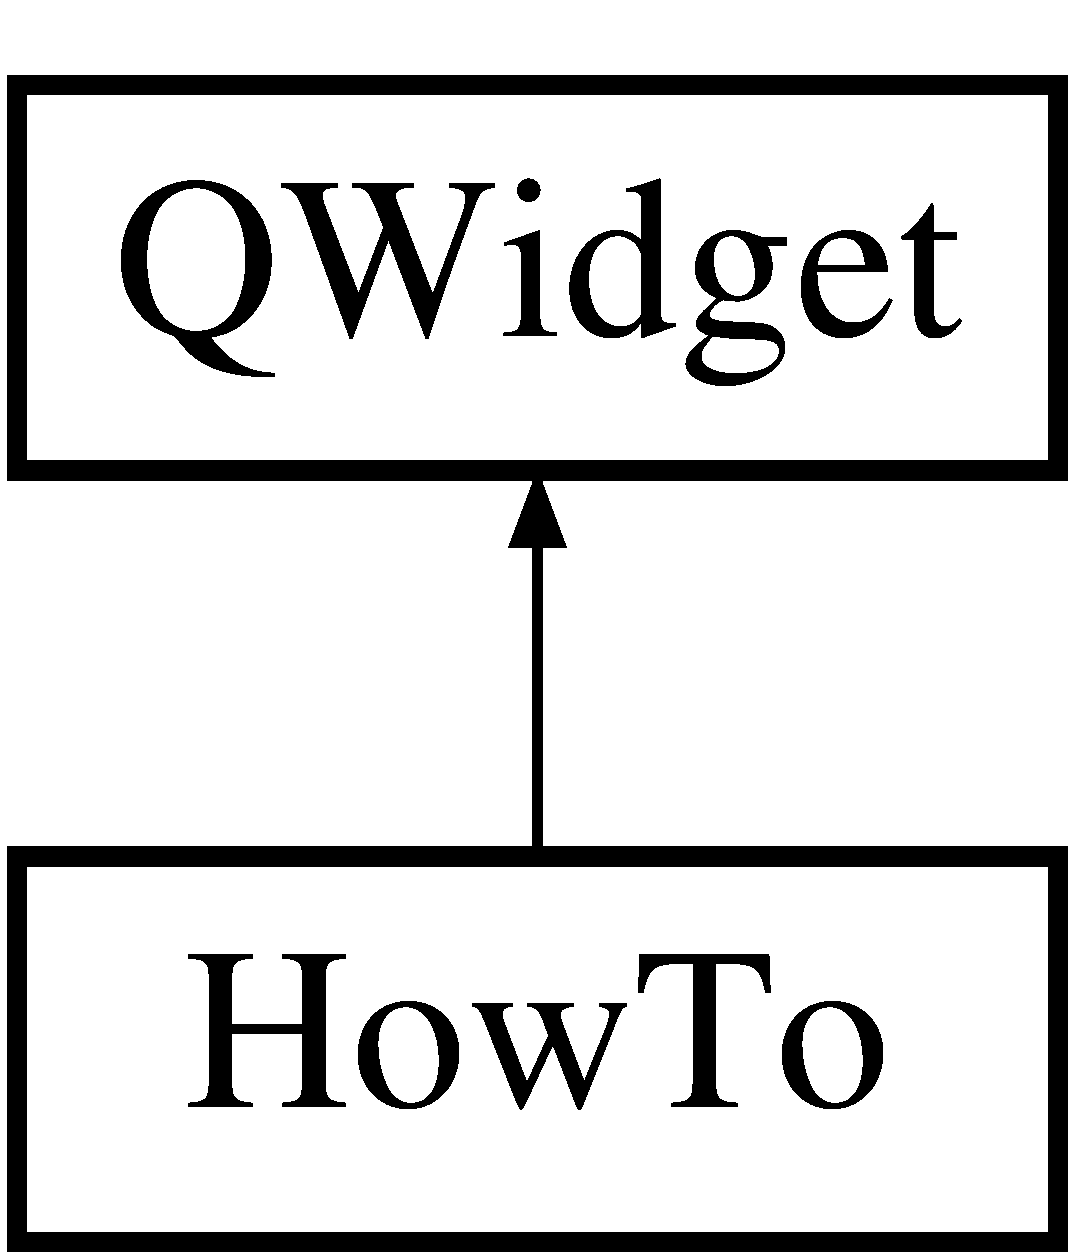
\includegraphics[height=2.000000cm]{class_how_to}
\end{center}
\end{figure}
\subsection*{Public Member Functions}
\begin{DoxyCompactItemize}
\item 
{\bf How\+To} (Q\+Widget $\ast$parent=0)
\item 
{\bf $\sim$\+How\+To} ()
\end{DoxyCompactItemize}


\subsection{Detailed Description}
The \doxyref{How\+To}{p.}{class_how_to} class displays controls for how the game is played~\newline
$\ast$ back closes \doxyref{How\+To}{p.}{class_how_to}, taking the user back to the \doxyref{Main\+Window}{p.}{class_main_window}. 

\subsection{Constructor \& Destructor Documentation}
\index{How\+To@{How\+To}!How\+To@{How\+To}}
\index{How\+To@{How\+To}!How\+To@{How\+To}}
\subsubsection[{How\+To}]{\setlength{\rightskip}{0pt plus 5cm}How\+To\+::\+How\+To (
\begin{DoxyParamCaption}
\item[{Q\+Widget $\ast$}]{parent = {\ttfamily 0}}
\end{DoxyParamCaption}
)\hspace{0.3cm}{\ttfamily [explicit]}}\label{class_how_to_aa35e11a42e32937aee2e4f5700ffd095}
\index{How\+To@{How\+To}!````~How\+To@{$\sim$\+How\+To}}
\index{````~How\+To@{$\sim$\+How\+To}!How\+To@{How\+To}}
\subsubsection[{$\sim$\+How\+To}]{\setlength{\rightskip}{0pt plus 5cm}How\+To\+::$\sim$\+How\+To (
\begin{DoxyParamCaption}
{}
\end{DoxyParamCaption}
)}\label{class_how_to_a704d3492bf6c31d651917ef3ec357256}


The documentation for this class was generated from the following files\+:\begin{DoxyCompactItemize}
\item 
Headers/{\bf howto.\+h}\item 
Sources/{\bf howto.\+cpp}\end{DoxyCompactItemize}

\section{Main\+Window Class Reference}
\label{class_main_window}\index{Main\+Window@{Main\+Window}}


The \doxyref{Main\+Window}{p.}{class_main_window} class displays the main menu for the game~\newline
$\ast$ board points to the \doxyref{Game\+Board}{p.}{class_game_board}~\newline
$\ast$ how points to the \doxyref{How\+To}{p.}{class_how_to}~\newline
$\ast$ quit points to the \doxyref{Quit\+Widget}{p.}{class_quit_widget}~\newline
$\ast$ title displays the title of the game~\newline
$\ast$ play takes the user to the game board~\newline
$\ast$ howto takes the user to the \doxyref{How\+To}{p.}{class_how_to} screen~\newline
$\ast$ exit brings up the \doxyref{Quit\+Widget}{p.}{class_quit_widget}~\newline
$\ast$ buttons stores the layout for the Q\+Push\+Button objects~\newline
$\ast$ final\+\_\+layout stores the final layout~\newline
$\ast$ central is the central widget applying final\+\_\+layout.  




{\ttfamily \#include $<$mainwindow.\+h$>$}

Inheritance diagram for Main\+Window\+:\begin{figure}[H]
\begin{center}
\leavevmode
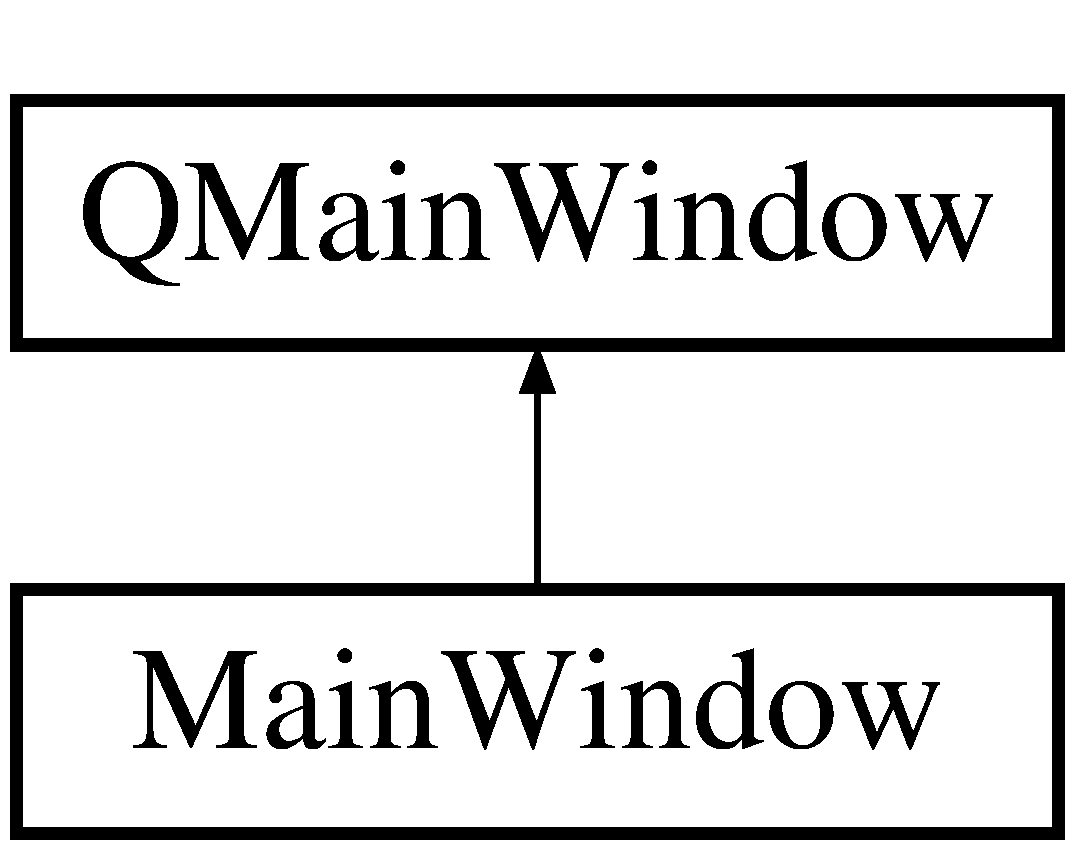
\includegraphics[height=2.000000cm]{class_main_window}
\end{center}
\end{figure}
\subsection*{Public Slots}
\begin{DoxyCompactItemize}
\item 
void {\bf make\+Game\+Board} ()
\begin{DoxyCompactList}\small\item\em make\+Game\+Board makes a new \doxyref{Game\+Board}{p.}{class_game_board} \end{DoxyCompactList}\end{DoxyCompactItemize}
\subsection*{Public Member Functions}
\begin{DoxyCompactItemize}
\item 
{\bf Main\+Window} (Q\+Widget $\ast$parent=0)
\item 
{\bf $\sim$\+Main\+Window} ()
\item 
void {\bf close\+Event} (Q\+Close\+Event $\ast$e)
\begin{DoxyCompactList}\small\item\em close\+Event shows \doxyref{Quit\+Widget}{p.}{class_quit_widget} when attempting to close \end{DoxyCompactList}\item 
void {\bf set\+How\+To} ({\bf How\+To} $\ast$how\+\_\+to)
\begin{DoxyCompactList}\small\item\em set\+Game\+Board sets \doxyref{Game\+Board}{p.}{class_game_board} \end{DoxyCompactList}\item 
void {\bf set\+Quit\+Widget} ({\bf Quit\+Widget} $\ast$quit\+\_\+widget)
\begin{DoxyCompactList}\small\item\em set\+Quit\+Widget sets \doxyref{Quit\+Widget}{p.}{class_quit_widget} \end{DoxyCompactList}\item 
void {\bf set\+Game\+Over\+Widget} ({\bf Game\+Over\+Widget} $\ast$game\+\_\+over)
\begin{DoxyCompactList}\small\item\em set\+Game\+Over\+Widget sets \doxyref{Game\+Over\+Widget}{p.}{class_game_over_widget} \end{DoxyCompactList}\end{DoxyCompactItemize}


\subsection{Detailed Description}
The \doxyref{Main\+Window}{p.}{class_main_window} class displays the main menu for the game~\newline
$\ast$ board points to the \doxyref{Game\+Board}{p.}{class_game_board}~\newline
$\ast$ how points to the \doxyref{How\+To}{p.}{class_how_to}~\newline
$\ast$ quit points to the \doxyref{Quit\+Widget}{p.}{class_quit_widget}~\newline
$\ast$ title displays the title of the game~\newline
$\ast$ play takes the user to the game board~\newline
$\ast$ howto takes the user to the \doxyref{How\+To}{p.}{class_how_to} screen~\newline
$\ast$ exit brings up the \doxyref{Quit\+Widget}{p.}{class_quit_widget}~\newline
$\ast$ buttons stores the layout for the Q\+Push\+Button objects~\newline
$\ast$ final\+\_\+layout stores the final layout~\newline
$\ast$ central is the central widget applying final\+\_\+layout. 

\subsection{Constructor \& Destructor Documentation}
\index{Main\+Window@{Main\+Window}!Main\+Window@{Main\+Window}}
\index{Main\+Window@{Main\+Window}!Main\+Window@{Main\+Window}}
\subsubsection[{Main\+Window}]{\setlength{\rightskip}{0pt plus 5cm}Main\+Window\+::\+Main\+Window (
\begin{DoxyParamCaption}
\item[{Q\+Widget $\ast$}]{parent = {\ttfamily 0}}
\end{DoxyParamCaption}
)\hspace{0.3cm}{\ttfamily [explicit]}}\label{class_main_window_a8b244be8b7b7db1b08de2a2acb9409db}
\index{Main\+Window@{Main\+Window}!````~Main\+Window@{$\sim$\+Main\+Window}}
\index{````~Main\+Window@{$\sim$\+Main\+Window}!Main\+Window@{Main\+Window}}
\subsubsection[{$\sim$\+Main\+Window}]{\setlength{\rightskip}{0pt plus 5cm}Main\+Window\+::$\sim$\+Main\+Window (
\begin{DoxyParamCaption}
{}
\end{DoxyParamCaption}
)}\label{class_main_window_ae98d00a93bc118200eeef9f9bba1dba7}


\subsection{Member Function Documentation}
\index{Main\+Window@{Main\+Window}!close\+Event@{close\+Event}}
\index{close\+Event@{close\+Event}!Main\+Window@{Main\+Window}}
\subsubsection[{close\+Event}]{\setlength{\rightskip}{0pt plus 5cm}void Main\+Window\+::close\+Event (
\begin{DoxyParamCaption}
\item[{Q\+Close\+Event $\ast$}]{e}
\end{DoxyParamCaption}
)}\label{class_main_window_a8a5bf36f9544ed3ec3a9eea9b7154564}


close\+Event shows \doxyref{Quit\+Widget}{p.}{class_quit_widget} when attempting to close 


\begin{DoxyParams}{Parameters}
{\em e} & unused \\
\hline
\end{DoxyParams}
\index{Main\+Window@{Main\+Window}!make\+Game\+Board@{make\+Game\+Board}}
\index{make\+Game\+Board@{make\+Game\+Board}!Main\+Window@{Main\+Window}}
\subsubsection[{make\+Game\+Board}]{\setlength{\rightskip}{0pt plus 5cm}void Main\+Window\+::make\+Game\+Board (
\begin{DoxyParamCaption}
{}
\end{DoxyParamCaption}
)\hspace{0.3cm}{\ttfamily [slot]}}\label{class_main_window_a0fffc2a0d1230e02a7fc402d665be9cc}


make\+Game\+Board makes a new \doxyref{Game\+Board}{p.}{class_game_board} 

\index{Main\+Window@{Main\+Window}!set\+Game\+Over\+Widget@{set\+Game\+Over\+Widget}}
\index{set\+Game\+Over\+Widget@{set\+Game\+Over\+Widget}!Main\+Window@{Main\+Window}}
\subsubsection[{set\+Game\+Over\+Widget}]{\setlength{\rightskip}{0pt plus 5cm}void Main\+Window\+::set\+Game\+Over\+Widget (
\begin{DoxyParamCaption}
\item[{{\bf Game\+Over\+Widget} $\ast$}]{game\+\_\+over}
\end{DoxyParamCaption}
)}\label{class_main_window_a1f5b83de288f1a1fe68999d06210b18b}


set\+Game\+Over\+Widget sets \doxyref{Game\+Over\+Widget}{p.}{class_game_over_widget} 


\begin{DoxyParams}{Parameters}
{\em game\+\_\+over} & the \doxyref{Game\+Over\+Widget}{p.}{class_game_over_widget} input \\
\hline
\end{DoxyParams}
\index{Main\+Window@{Main\+Window}!set\+How\+To@{set\+How\+To}}
\index{set\+How\+To@{set\+How\+To}!Main\+Window@{Main\+Window}}
\subsubsection[{set\+How\+To}]{\setlength{\rightskip}{0pt plus 5cm}void Main\+Window\+::set\+How\+To (
\begin{DoxyParamCaption}
\item[{{\bf How\+To} $\ast$}]{how\+\_\+to}
\end{DoxyParamCaption}
)}\label{class_main_window_ae30bf0fbea2927e74edda8b49aaacb21}


set\+Game\+Board sets \doxyref{Game\+Board}{p.}{class_game_board} 


\begin{DoxyParams}{Parameters}
{\em game\+\_\+board} & the \doxyref{Game\+Board}{p.}{class_game_board} input set\+How\+To sets \doxyref{How\+To}{p.}{class_how_to} \\
\hline
{\em how\+\_\+to} & the \doxyref{How\+To}{p.}{class_how_to} input \\
\hline
\end{DoxyParams}
\index{Main\+Window@{Main\+Window}!set\+Quit\+Widget@{set\+Quit\+Widget}}
\index{set\+Quit\+Widget@{set\+Quit\+Widget}!Main\+Window@{Main\+Window}}
\subsubsection[{set\+Quit\+Widget}]{\setlength{\rightskip}{0pt plus 5cm}void Main\+Window\+::set\+Quit\+Widget (
\begin{DoxyParamCaption}
\item[{{\bf Quit\+Widget} $\ast$}]{quit\+\_\+widget}
\end{DoxyParamCaption}
)}\label{class_main_window_a7a21783f6de547af62faad76b83fb0d7}


set\+Quit\+Widget sets \doxyref{Quit\+Widget}{p.}{class_quit_widget} 


\begin{DoxyParams}{Parameters}
{\em quit\+\_\+widget} & the \doxyref{Quit\+Widget}{p.}{class_quit_widget} input \\
\hline
\end{DoxyParams}


The documentation for this class was generated from the following files\+:\begin{DoxyCompactItemize}
\item 
Headers/{\bf mainwindow.\+h}\item 
Sources/{\bf mainwindow.\+cpp}\end{DoxyCompactItemize}

\section{Pikachu Class Reference}
\label{class_pikachu}\index{Pikachu@{Pikachu}}


The \doxyref{Pikachu}{p.}{class_pikachu} class is the user controlled \doxyref{Pikachu}{p.}{class_pikachu}~\newline
 x, y store the coordinates~\newline
 int lives stores the number of lives~\newline
 int max\+\_\+lives stores the max number of lives~\newline
 int dir represents direction (0 = up, 1 = down, 2 = left, 3 = right)~\newline
$\ast$ up\+\_\+image stores the facing up image~\newline
$\ast$ down\+\_\+image stores the facing down image~\newline
$\ast$ left\+\_\+image stores the facing left image~\newline
$\ast$ right\+\_\+image stores the facing right image.  




{\ttfamily \#include $<$pikachu.\+h$>$}

\subsection*{Public Member Functions}
\begin{DoxyCompactItemize}
\item 
{\bf Pikachu} ()
\item 
int {\bf get\+\_\+x} ()
\begin{DoxyCompactList}\small\item\em get\+\_\+x returns x \end{DoxyCompactList}\item 
int {\bf get\+\_\+y} ()
\begin{DoxyCompactList}\small\item\em get\+\_\+y returns y \end{DoxyCompactList}\item 
int {\bf get\+\_\+dir} ()
\begin{DoxyCompactList}\small\item\em get\+\_\+dir returns dir \end{DoxyCompactList}\item 
void {\bf set\+\_\+x} (int nx)
\begin{DoxyCompactList}\small\item\em set\+\_\+x sets x \end{DoxyCompactList}\item 
void {\bf set\+\_\+y} (int ny)
\begin{DoxyCompactList}\small\item\em set\+\_\+y sets y \end{DoxyCompactList}\item 
void {\bf set\+\_\+dir} (int d)
\begin{DoxyCompactList}\small\item\em set\+\_\+dir sets dir \end{DoxyCompactList}\item 
unsigned int {\bf get\+\_\+lives} ()
\begin{DoxyCompactList}\small\item\em get\+\_\+lives returns lives \end{DoxyCompactList}\item 
void {\bf lose\+\_\+life} ()
\begin{DoxyCompactList}\small\item\em lose\+\_\+life decrements lives \end{DoxyCompactList}\item 
void {\bf gain\+\_\+life} ()
\begin{DoxyCompactList}\small\item\em gain\+\_\+life increments lives \end{DoxyCompactList}\item 
Q\+Pixmap $\ast$ {\bf get\+\_\+up\+\_\+image} ()
\begin{DoxyCompactList}\small\item\em get\+\_\+up\+\_\+image returns up\+\_\+image \end{DoxyCompactList}\item 
Q\+Pixmap $\ast$ {\bf get\+\_\+down\+\_\+image} ()
\begin{DoxyCompactList}\small\item\em get\+\_\+down\+\_\+image returns down\+\_\+image \end{DoxyCompactList}\item 
Q\+Pixmap $\ast$ {\bf get\+\_\+left\+\_\+image} ()
\begin{DoxyCompactList}\small\item\em get\+\_\+left\+\_\+image returns left\+\_\+image \end{DoxyCompactList}\item 
Q\+Pixmap $\ast$ {\bf get\+\_\+right\+\_\+image} ()
\begin{DoxyCompactList}\small\item\em get\+\_\+right\+\_\+image returns right\+\_\+image \end{DoxyCompactList}\item 
{\bf $\sim$\+Pikachu} ()
\end{DoxyCompactItemize}


\subsection{Detailed Description}
The \doxyref{Pikachu}{p.}{class_pikachu} class is the user controlled \doxyref{Pikachu}{p.}{class_pikachu}~\newline
 x, y store the coordinates~\newline
 int lives stores the number of lives~\newline
 int max\+\_\+lives stores the max number of lives~\newline
 int dir represents direction (0 = up, 1 = down, 2 = left, 3 = right)~\newline
$\ast$ up\+\_\+image stores the facing up image~\newline
$\ast$ down\+\_\+image stores the facing down image~\newline
$\ast$ left\+\_\+image stores the facing left image~\newline
$\ast$ right\+\_\+image stores the facing right image. 

\subsection{Constructor \& Destructor Documentation}
\index{Pikachu@{Pikachu}!Pikachu@{Pikachu}}
\index{Pikachu@{Pikachu}!Pikachu@{Pikachu}}
\subsubsection[{Pikachu}]{\setlength{\rightskip}{0pt plus 5cm}Pikachu\+::\+Pikachu (
\begin{DoxyParamCaption}
{}
\end{DoxyParamCaption}
)}\label{class_pikachu_a0305d1eb9d3c37309a50dbff620dee76}
\index{Pikachu@{Pikachu}!````~Pikachu@{$\sim$\+Pikachu}}
\index{````~Pikachu@{$\sim$\+Pikachu}!Pikachu@{Pikachu}}
\subsubsection[{$\sim$\+Pikachu}]{\setlength{\rightskip}{0pt plus 5cm}Pikachu\+::$\sim$\+Pikachu (
\begin{DoxyParamCaption}
{}
\end{DoxyParamCaption}
)}\label{class_pikachu_a83f883a1354d3a387363f2bee8f19a4f}


\subsection{Member Function Documentation}
\index{Pikachu@{Pikachu}!gain\+\_\+life@{gain\+\_\+life}}
\index{gain\+\_\+life@{gain\+\_\+life}!Pikachu@{Pikachu}}
\subsubsection[{gain\+\_\+life}]{\setlength{\rightskip}{0pt plus 5cm}void Pikachu\+::gain\+\_\+life (
\begin{DoxyParamCaption}
{}
\end{DoxyParamCaption}
)}\label{class_pikachu_adebcbf638d3c4c6b5df59c02e29b0fd9}


gain\+\_\+life increments lives 

\index{Pikachu@{Pikachu}!get\+\_\+dir@{get\+\_\+dir}}
\index{get\+\_\+dir@{get\+\_\+dir}!Pikachu@{Pikachu}}
\subsubsection[{get\+\_\+dir}]{\setlength{\rightskip}{0pt plus 5cm}int Pikachu\+::get\+\_\+dir (
\begin{DoxyParamCaption}
{}
\end{DoxyParamCaption}
)}\label{class_pikachu_ae04801873c0bfb824b315c71420fff07}


get\+\_\+dir returns dir 

\begin{DoxyReturn}{Returns}
dir 
\end{DoxyReturn}
\index{Pikachu@{Pikachu}!get\+\_\+down\+\_\+image@{get\+\_\+down\+\_\+image}}
\index{get\+\_\+down\+\_\+image@{get\+\_\+down\+\_\+image}!Pikachu@{Pikachu}}
\subsubsection[{get\+\_\+down\+\_\+image}]{\setlength{\rightskip}{0pt plus 5cm}Q\+Pixmap $\ast$ Pikachu\+::get\+\_\+down\+\_\+image (
\begin{DoxyParamCaption}
{}
\end{DoxyParamCaption}
)}\label{class_pikachu_a7a57ef922c7f1e5f86ee7e85b635a833}


get\+\_\+down\+\_\+image returns down\+\_\+image 

\begin{DoxyReturn}{Returns}
down\+\_\+image 
\end{DoxyReturn}
\index{Pikachu@{Pikachu}!get\+\_\+left\+\_\+image@{get\+\_\+left\+\_\+image}}
\index{get\+\_\+left\+\_\+image@{get\+\_\+left\+\_\+image}!Pikachu@{Pikachu}}
\subsubsection[{get\+\_\+left\+\_\+image}]{\setlength{\rightskip}{0pt plus 5cm}Q\+Pixmap $\ast$ Pikachu\+::get\+\_\+left\+\_\+image (
\begin{DoxyParamCaption}
{}
\end{DoxyParamCaption}
)}\label{class_pikachu_ad838cedcdbaecc1e5d3ff37842bcc72f}


get\+\_\+left\+\_\+image returns left\+\_\+image 

\begin{DoxyReturn}{Returns}
left\+\_\+image 
\end{DoxyReturn}
\index{Pikachu@{Pikachu}!get\+\_\+lives@{get\+\_\+lives}}
\index{get\+\_\+lives@{get\+\_\+lives}!Pikachu@{Pikachu}}
\subsubsection[{get\+\_\+lives}]{\setlength{\rightskip}{0pt plus 5cm}unsigned int Pikachu\+::get\+\_\+lives (
\begin{DoxyParamCaption}
{}
\end{DoxyParamCaption}
)}\label{class_pikachu_abada106a76f29708793c28e66076d6eb}


get\+\_\+lives returns lives 

\begin{DoxyReturn}{Returns}
lives 
\end{DoxyReturn}
\index{Pikachu@{Pikachu}!get\+\_\+right\+\_\+image@{get\+\_\+right\+\_\+image}}
\index{get\+\_\+right\+\_\+image@{get\+\_\+right\+\_\+image}!Pikachu@{Pikachu}}
\subsubsection[{get\+\_\+right\+\_\+image}]{\setlength{\rightskip}{0pt plus 5cm}Q\+Pixmap $\ast$ Pikachu\+::get\+\_\+right\+\_\+image (
\begin{DoxyParamCaption}
{}
\end{DoxyParamCaption}
)}\label{class_pikachu_a22acb20e14e3ee754c0867aec461c961}


get\+\_\+right\+\_\+image returns right\+\_\+image 

\begin{DoxyReturn}{Returns}
right\+\_\+image 
\end{DoxyReturn}
\index{Pikachu@{Pikachu}!get\+\_\+up\+\_\+image@{get\+\_\+up\+\_\+image}}
\index{get\+\_\+up\+\_\+image@{get\+\_\+up\+\_\+image}!Pikachu@{Pikachu}}
\subsubsection[{get\+\_\+up\+\_\+image}]{\setlength{\rightskip}{0pt plus 5cm}Q\+Pixmap $\ast$ Pikachu\+::get\+\_\+up\+\_\+image (
\begin{DoxyParamCaption}
{}
\end{DoxyParamCaption}
)}\label{class_pikachu_ab4d821dd315e41907b23fce3c79d82f4}


get\+\_\+up\+\_\+image returns up\+\_\+image 

\begin{DoxyReturn}{Returns}
up\+\_\+image 
\end{DoxyReturn}
\index{Pikachu@{Pikachu}!get\+\_\+x@{get\+\_\+x}}
\index{get\+\_\+x@{get\+\_\+x}!Pikachu@{Pikachu}}
\subsubsection[{get\+\_\+x}]{\setlength{\rightskip}{0pt plus 5cm}int Pikachu\+::get\+\_\+x (
\begin{DoxyParamCaption}
{}
\end{DoxyParamCaption}
)}\label{class_pikachu_a1be8e1ab99ff544e454ea9308004f9d9}


get\+\_\+x returns x 

\begin{DoxyReturn}{Returns}
x 
\end{DoxyReturn}
\index{Pikachu@{Pikachu}!get\+\_\+y@{get\+\_\+y}}
\index{get\+\_\+y@{get\+\_\+y}!Pikachu@{Pikachu}}
\subsubsection[{get\+\_\+y}]{\setlength{\rightskip}{0pt plus 5cm}int Pikachu\+::get\+\_\+y (
\begin{DoxyParamCaption}
{}
\end{DoxyParamCaption}
)}\label{class_pikachu_adc0a555fbb343fb357ac8284a44904c6}


get\+\_\+y returns y 

\begin{DoxyReturn}{Returns}
y 
\end{DoxyReturn}
\index{Pikachu@{Pikachu}!lose\+\_\+life@{lose\+\_\+life}}
\index{lose\+\_\+life@{lose\+\_\+life}!Pikachu@{Pikachu}}
\subsubsection[{lose\+\_\+life}]{\setlength{\rightskip}{0pt plus 5cm}void Pikachu\+::lose\+\_\+life (
\begin{DoxyParamCaption}
{}
\end{DoxyParamCaption}
)}\label{class_pikachu_aa40dc8df907b10c01da9948053fe0d86}


lose\+\_\+life decrements lives 

\index{Pikachu@{Pikachu}!set\+\_\+dir@{set\+\_\+dir}}
\index{set\+\_\+dir@{set\+\_\+dir}!Pikachu@{Pikachu}}
\subsubsection[{set\+\_\+dir}]{\setlength{\rightskip}{0pt plus 5cm}void Pikachu\+::set\+\_\+dir (
\begin{DoxyParamCaption}
\item[{int}]{d}
\end{DoxyParamCaption}
)}\label{class_pikachu_aaa1f2ed8cc4bdc41e47bbcbff0fc108b}


set\+\_\+dir sets dir 


\begin{DoxyParams}{Parameters}
{\em d} & the input dir \\
\hline
\end{DoxyParams}
\index{Pikachu@{Pikachu}!set\+\_\+x@{set\+\_\+x}}
\index{set\+\_\+x@{set\+\_\+x}!Pikachu@{Pikachu}}
\subsubsection[{set\+\_\+x}]{\setlength{\rightskip}{0pt plus 5cm}void Pikachu\+::set\+\_\+x (
\begin{DoxyParamCaption}
\item[{int}]{nx}
\end{DoxyParamCaption}
)}\label{class_pikachu_a7fb60ef90f71080fd00ca4afb330ace2}


set\+\_\+x sets x 


\begin{DoxyParams}{Parameters}
{\em nx} & the input x coordinate \\
\hline
\end{DoxyParams}
\index{Pikachu@{Pikachu}!set\+\_\+y@{set\+\_\+y}}
\index{set\+\_\+y@{set\+\_\+y}!Pikachu@{Pikachu}}
\subsubsection[{set\+\_\+y}]{\setlength{\rightskip}{0pt plus 5cm}void Pikachu\+::set\+\_\+y (
\begin{DoxyParamCaption}
\item[{int}]{ny}
\end{DoxyParamCaption}
)}\label{class_pikachu_a086d84dea037a532056b51eefc166d5a}


set\+\_\+y sets y 


\begin{DoxyParams}{Parameters}
{\em ny} & the input y coordinate \\
\hline
\end{DoxyParams}


The documentation for this class was generated from the following files\+:\begin{DoxyCompactItemize}
\item 
Headers/{\bf pikachu.\+h}\item 
Sources/{\bf pikachu.\+cpp}\end{DoxyCompactItemize}

\section{Quit\+Widget Class Reference}
\label{class_quit_widget}\index{Quit\+Widget@{Quit\+Widget}}


The \doxyref{Quit\+Widget}{p.}{class_quit_widget} class displays the confirmation message upon exit~\newline
$\ast$ ok closes the application when clicked~\newline
$\ast$ sure displays the confirmation message~\newline
$\ast$ cancel returns the user to the main menu.  




{\ttfamily \#include $<$quitwidget.\+h$>$}

Inheritance diagram for Quit\+Widget\+:\begin{figure}[H]
\begin{center}
\leavevmode
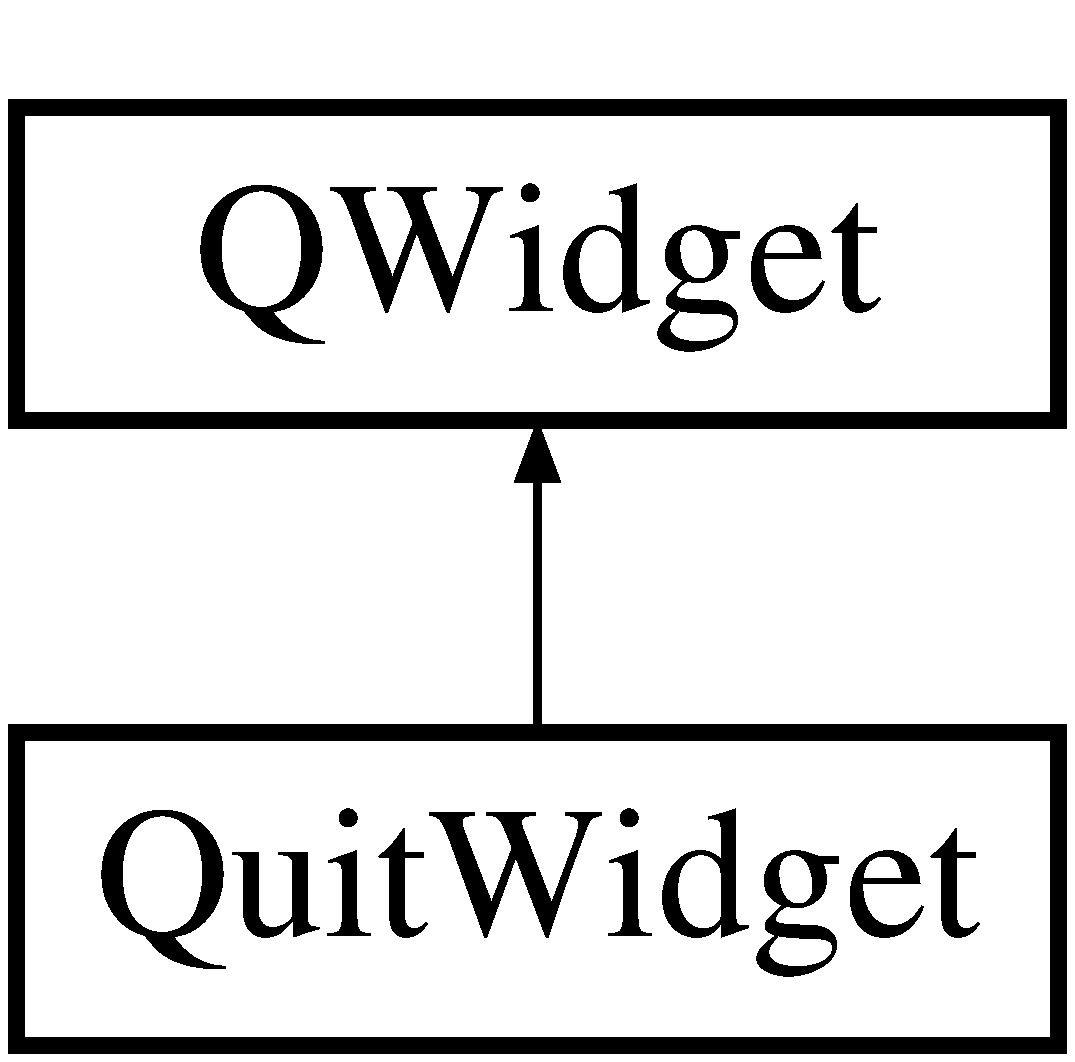
\includegraphics[height=2.000000cm]{class_quit_widget}
\end{center}
\end{figure}
\subsection*{Public Member Functions}
\begin{DoxyCompactItemize}
\item 
{\bf Quit\+Widget} (Q\+Widget $\ast$parent=0)
\item 
{\bf $\sim$\+Quit\+Widget} ()
\end{DoxyCompactItemize}
\subsection*{Public Attributes}
\begin{DoxyCompactItemize}
\item 
Q\+Push\+Button $\ast$ {\bf ok}
\end{DoxyCompactItemize}


\subsection{Detailed Description}
The \doxyref{Quit\+Widget}{p.}{class_quit_widget} class displays the confirmation message upon exit~\newline
$\ast$ ok closes the application when clicked~\newline
$\ast$ sure displays the confirmation message~\newline
$\ast$ cancel returns the user to the main menu. 

\subsection{Constructor \& Destructor Documentation}
\index{Quit\+Widget@{Quit\+Widget}!Quit\+Widget@{Quit\+Widget}}
\index{Quit\+Widget@{Quit\+Widget}!Quit\+Widget@{Quit\+Widget}}
\subsubsection[{Quit\+Widget}]{\setlength{\rightskip}{0pt plus 5cm}Quit\+Widget\+::\+Quit\+Widget (
\begin{DoxyParamCaption}
\item[{Q\+Widget $\ast$}]{parent = {\ttfamily 0}}
\end{DoxyParamCaption}
)\hspace{0.3cm}{\ttfamily [explicit]}}\label{class_quit_widget_a13ba091406c4c569e968f0ff5bd8105e}
\index{Quit\+Widget@{Quit\+Widget}!````~Quit\+Widget@{$\sim$\+Quit\+Widget}}
\index{````~Quit\+Widget@{$\sim$\+Quit\+Widget}!Quit\+Widget@{Quit\+Widget}}
\subsubsection[{$\sim$\+Quit\+Widget}]{\setlength{\rightskip}{0pt plus 5cm}Quit\+Widget\+::$\sim$\+Quit\+Widget (
\begin{DoxyParamCaption}
{}
\end{DoxyParamCaption}
)}\label{class_quit_widget_af6bbaf30e73f13a82998c8931a722904}


\subsection{Member Data Documentation}
\index{Quit\+Widget@{Quit\+Widget}!ok@{ok}}
\index{ok@{ok}!Quit\+Widget@{Quit\+Widget}}
\subsubsection[{ok}]{\setlength{\rightskip}{0pt plus 5cm}Q\+Push\+Button$\ast$ Quit\+Widget\+::ok}\label{class_quit_widget_a9d7b9c211c5a117c89050f2e372402e1}


The documentation for this class was generated from the following files\+:\begin{DoxyCompactItemize}
\item 
Headers/{\bf quitwidget.\+h}\item 
Sources/{\bf quitwidget.\+cpp}\end{DoxyCompactItemize}

\chapter{File Documentation}
\section{Headers/gameboard.h File Reference}
\label{gameboard_8h}\index{Headers/gameboard.\+h@{Headers/gameboard.\+h}}
{\ttfamily \#include \char`\"{}gameoverwidget.\+h\char`\"{}}\\*
{\ttfamily \#include \char`\"{}mainwindow.\+h\char`\"{}}\\*
{\ttfamily \#include \char`\"{}pikachu.\+h\char`\"{}}\\*
{\ttfamily \#include \char`\"{}quitwidget.\+h\char`\"{}}\\*
{\ttfamily \#include $<$Q\+Core\+Application$>$}\\*
{\ttfamily \#include $<$Q\+Cursor$>$}\\*
{\ttfamily \#include $<$Q\+Key\+Event$>$}\\*
{\ttfamily \#include $<$Q\+Mouse\+Event$>$}\\*
{\ttfamily \#include $<$Q\+Pixmap$>$}\\*
{\ttfamily \#include $<$Q\+Point$>$}\\*
{\ttfamily \#include $<$Q\+Rect$>$}\\*
{\ttfamily \#include $<$Q\+String$>$}\\*
{\ttfamily \#include $<$Q\+Widget$>$}\\*
{\ttfamily \#include $<$Q\+Timer$>$}\\*
{\ttfamily \#include $<$chrono$>$}\\*
{\ttfamily \#include $<$cmath$>$}\\*
{\ttfamily \#include $<$random$>$}\\*
{\ttfamily \#include $<$thread$>$}\\*
{\ttfamily \#include $<$vector$>$}\\*
\subsection*{Classes}
\begin{DoxyCompactItemize}
\item 
class {\bf Game\+Board}
\begin{DoxyCompactList}\small\item\em The \doxyref{Game\+Board}{p.}{class_game_board} class displays the board on which the game is played~\newline
$\ast$ Top displays the lives and score~\newline
$\ast$$\ast$ lives stores pointers to Q\+Label objects displaying the images for each life~\newline
$\ast$ score\+\_\+label displays the score~\newline
 int score stores the score~\newline
$\ast$ Board displays the tiles~\newline
$\ast$$\ast$ labels stores pointers to Q\+Label objects displaying each tile~\newline
 board\+\_\+size stores the size of the board~\newline
 cursor\+\_\+location stores the location of the cursor~\newline
 life\+\_\+position stores the location of the extra life~\newline
 clicked stores whether the mouse was clicked~\newline
$\ast$ squirtle\+\_\+image stores the image of the squirtles~\newline
$\ast$ charmander\+\_\+image stores the image of the charmanders~\newline
$\ast$ attack\+\_\+image stores the image of the attack~\newline
 number\+\_\+squirtles stores the total number of squirtles on the board~\newline
 alive\+\_\+squirtles stores the number of squirtles that have yet to be defeated~\newline
 number\+\_\+charmanders stores the total number of charmanders on the board~\newline
 alive\+\_\+charmanders stores the number of charmanders that have yet to be defeated~\newline
$\ast$ q points to the \doxyref{Quit\+Widget}{p.}{class_quit_widget} object~\newline
$\ast$ m points to the \doxyref{Main\+Window}{p.}{class_main_window} object~\newline
$\ast$ g points to the \doxyref{Game\+Over\+Widget}{p.}{class_game_over_widget} object~\newline
$\ast$ pika points to the \doxyref{Pikachu}{p.}{class_pikachu} object controlled by the player. \end{DoxyCompactList}\end{DoxyCompactItemize}

\section{Headers/gameoverwidget.h File Reference}
\label{gameoverwidget_8h}\index{Headers/gameoverwidget.\+h@{Headers/gameoverwidget.\+h}}
{\ttfamily \#include \char`\"{}gameboard.\+h\char`\"{}}\\*
{\ttfamily \#include \char`\"{}mainwindow.\+h\char`\"{}}\\*
{\ttfamily \#include \char`\"{}quitwidget.\+h\char`\"{}}\\*
{\ttfamily \#include $<$Q\+Box\+Layout$>$}\\*
{\ttfamily \#include $<$Q\+Label$>$}\\*
{\ttfamily \#include $<$Q\+Push\+Button$>$}\\*
{\ttfamily \#include $<$Q\+Widget$>$}\\*
\subsection*{Classes}
\begin{DoxyCompactItemize}
\item 
class {\bf Game\+Over\+Widget}
\begin{DoxyCompactList}\small\item\em The \doxyref{Game\+Over\+Widget}{p.}{class_game_over_widget} class~\newline
$\ast$ over displays the \char`\"{}\+Game Over!\char`\"{} message~\newline
$\ast$ play\+Again takes the user to a new game~\newline
$\ast$ main\+Menu takes the user to the main menu~\newline
$\ast$ exit brings up the \doxyref{Quit\+Widget}{p.}{class_quit_widget}~\newline
$\ast$ mw points to the \doxyref{Main\+Window}{p.}{class_main_window}~\newline
$\ast$ board points to the \doxyref{Game\+Board}{p.}{class_game_board}~\newline
$\ast$ quit points to the \doxyref{Quit\+Widget}{p.}{class_quit_widget}. \end{DoxyCompactList}\end{DoxyCompactItemize}

\section{Headers/howto.h File Reference}
\label{howto_8h}\index{Headers/howto.\+h@{Headers/howto.\+h}}
{\ttfamily \#include \char`\"{}mainwindow.\+h\char`\"{}}\\*
{\ttfamily \#include \char`\"{}quitwidget.\+h\char`\"{}}\\*
{\ttfamily \#include $<$Q\+Box\+Layout$>$}\\*
{\ttfamily \#include $<$Q\+Label$>$}\\*
{\ttfamily \#include $<$Q\+Widget$>$}\\*
\subsection*{Classes}
\begin{DoxyCompactItemize}
\item 
class {\bf How\+To}
\begin{DoxyCompactList}\small\item\em The \doxyref{How\+To}{p.}{class_how_to} class displays controls for how the game is played~\newline
$\ast$ back closes \doxyref{How\+To}{p.}{class_how_to}, taking the user back to the \doxyref{Main\+Window}{p.}{class_main_window}. \end{DoxyCompactList}\end{DoxyCompactItemize}

\section{Headers/mainwindow.h File Reference}
\label{mainwindow_8h}\index{Headers/mainwindow.\+h@{Headers/mainwindow.\+h}}
{\ttfamily \#include \char`\"{}gameboard.\+h\char`\"{}}\\*
{\ttfamily \#include \char`\"{}gameoverwidget.\+h\char`\"{}}\\*
{\ttfamily \#include \char`\"{}howto.\+h\char`\"{}}\\*
{\ttfamily \#include \char`\"{}quitwidget.\+h\char`\"{}}\\*
{\ttfamily \#include $<$Q\+Font$>$}\\*
{\ttfamily \#include $<$Q\+Label$>$}\\*
{\ttfamily \#include $<$Q\+Main\+Window$>$}\\*
{\ttfamily \#include $<$Q\+Push\+Button$>$}\\*
{\ttfamily \#include $<$Q\+V\+Box\+Layout$>$}\\*
\subsection*{Classes}
\begin{DoxyCompactItemize}
\item 
class {\bf Main\+Window}
\begin{DoxyCompactList}\small\item\em The \doxyref{Main\+Window}{p.}{class_main_window} class displays the main menu for the game~\newline
$\ast$ board points to the \doxyref{Game\+Board}{p.}{class_game_board}~\newline
$\ast$ how points to the \doxyref{How\+To}{p.}{class_how_to}~\newline
$\ast$ quit points to the \doxyref{Quit\+Widget}{p.}{class_quit_widget}~\newline
$\ast$ title displays the title of the game~\newline
$\ast$ play takes the user to the game board~\newline
$\ast$ howto takes the user to the \doxyref{How\+To}{p.}{class_how_to} screen~\newline
$\ast$ exit brings up the \doxyref{Quit\+Widget}{p.}{class_quit_widget}~\newline
$\ast$ buttons stores the layout for the Q\+Push\+Button objects~\newline
$\ast$ final\+\_\+layout stores the final layout~\newline
$\ast$ central is the central widget applying final\+\_\+layout. \end{DoxyCompactList}\end{DoxyCompactItemize}

\section{Headers/pikachu.h File Reference}
\label{pikachu_8h}\index{Headers/pikachu.\+h@{Headers/pikachu.\+h}}
{\ttfamily \#include $<$Q\+Label$>$}\\*
\subsection*{Classes}
\begin{DoxyCompactItemize}
\item 
class {\bf Pikachu}
\begin{DoxyCompactList}\small\item\em The \doxyref{Pikachu}{p.}{class_pikachu} class is the user controlled \doxyref{Pikachu}{p.}{class_pikachu}~\newline
 x, y store the coordinates~\newline
 int lives stores the number of lives~\newline
 int max\+\_\+lives stores the max number of lives~\newline
 int dir represents direction (0 = up, 1 = down, 2 = left, 3 = right)~\newline
$\ast$ up\+\_\+image stores the facing up image~\newline
$\ast$ down\+\_\+image stores the facing down image~\newline
$\ast$ left\+\_\+image stores the facing left image~\newline
$\ast$ right\+\_\+image stores the facing right image. \end{DoxyCompactList}\end{DoxyCompactItemize}

\section{Headers/quitwidget.h File Reference}
\label{quitwidget_8h}\index{Headers/quitwidget.\+h@{Headers/quitwidget.\+h}}
{\ttfamily \#include $<$Q\+Box\+Layout$>$}\\*
{\ttfamily \#include $<$Q\+Label$>$}\\*
{\ttfamily \#include $<$Q\+Push\+Button$>$}\\*
{\ttfamily \#include $<$Q\+Widget$>$}\\*
\subsection*{Classes}
\begin{DoxyCompactItemize}
\item 
class {\bf Quit\+Widget}
\begin{DoxyCompactList}\small\item\em The \doxyref{Quit\+Widget}{p.}{class_quit_widget} class displays the confirmation message upon exit~\newline
$\ast$ ok closes the application when clicked~\newline
$\ast$ sure displays the confirmation message~\newline
$\ast$ cancel returns the user to the main menu. \end{DoxyCompactList}\end{DoxyCompactItemize}

\section{Sources/gameboard.cpp File Reference}
\label{gameboard_8cpp}\index{Sources/gameboard.\+cpp@{Sources/gameboard.\+cpp}}
{\ttfamily \#include \char`\"{}..\textbackslash{}\+Headers\textbackslash{}gameboard.\+h\char`\"{}}\\*
\subsection*{Functions}
\begin{DoxyCompactItemize}
\item 
std\+::default\+\_\+random\+\_\+engine {\bf generator} ({\bf seed})
\end{DoxyCompactItemize}
\subsection*{Variables}
\begin{DoxyCompactItemize}
\item 
unsigned {\bf seed} = std\+::chrono\+::system\+\_\+clock\+::now().time\+\_\+since\+\_\+epoch().count()
\end{DoxyCompactItemize}


\subsection{Function Documentation}
\index{gameboard.\+cpp@{gameboard.\+cpp}!generator@{generator}}
\index{generator@{generator}!gameboard.\+cpp@{gameboard.\+cpp}}
\subsubsection[{generator}]{\setlength{\rightskip}{0pt plus 5cm}std\+::default\+\_\+random\+\_\+engine generator (
\begin{DoxyParamCaption}
\item[{{\bf seed}}]{}
\end{DoxyParamCaption}
)}\label{gameboard_8cpp_a7739f9a14ee87e088af1af3ba2bdada3}


\subsection{Variable Documentation}
\index{gameboard.\+cpp@{gameboard.\+cpp}!seed@{seed}}
\index{seed@{seed}!gameboard.\+cpp@{gameboard.\+cpp}}
\subsubsection[{seed}]{\setlength{\rightskip}{0pt plus 5cm}unsigned seed = std\+::chrono\+::system\+\_\+clock\+::now().time\+\_\+since\+\_\+epoch().count()}\label{gameboard_8cpp_abb3c5a016eb55b340002c5da33a16714}

\section{Sources/gameoverwidget.cpp File Reference}
\label{gameoverwidget_8cpp}\index{Sources/gameoverwidget.\+cpp@{Sources/gameoverwidget.\+cpp}}
{\ttfamily \#include \char`\"{}..\textbackslash{}\+Headers\textbackslash{}gameoverwidget.\+h\char`\"{}}\\*

\section{Sources/howto.cpp File Reference}
\label{howto_8cpp}\index{Sources/howto.\+cpp@{Sources/howto.\+cpp}}
{\ttfamily \#include \char`\"{}..\textbackslash{}\+Headers\textbackslash{}howto.\+h\char`\"{}}\\*

\section{Sources/main.cpp File Reference}
\label{main_8cpp}\index{Sources/main.\+cpp@{Sources/main.\+cpp}}
{\ttfamily \#include \char`\"{}..\textbackslash{}\+Headers\textbackslash{}mainwindow.\+h\char`\"{}}\\*
{\ttfamily \#include \char`\"{}..\textbackslash{}\+Headers\textbackslash{}quitwidget.\+h\char`\"{}}\\*
{\ttfamily \#include \char`\"{}..\textbackslash{}\+Headers\textbackslash{}gameboard.\+h\char`\"{}}\\*
{\ttfamily \#include \char`\"{}..\textbackslash{}\+Headers\textbackslash{}howto.\+h\char`\"{}}\\*
{\ttfamily \#include \char`\"{}..\textbackslash{}\+Headers\textbackslash{}gameoverwidget.\+h\char`\"{}}\\*
{\ttfamily \#include $<$Q\+Application$>$}\\*
\subsection*{Functions}
\begin{DoxyCompactItemize}
\item 
int {\bf main} (int argc, char $\ast$argv[$\,$])
\end{DoxyCompactItemize}


\subsection{Function Documentation}
\index{main.\+cpp@{main.\+cpp}!main@{main}}
\index{main@{main}!main.\+cpp@{main.\+cpp}}
\subsubsection[{main}]{\setlength{\rightskip}{0pt plus 5cm}int main (
\begin{DoxyParamCaption}
\item[{int}]{argc, }
\item[{char $\ast$}]{argv[$\,$]}
\end{DoxyParamCaption}
)}\label{main_8cpp_a0ddf1224851353fc92bfbff6f499fa97}
Joshua Cheung P\+I\+C 10\+C Discussion 1\+A 11/14/14 A tile-\/based game in which the objective is to defeat a number of enemies 
\section{Sources/mainwindow.cpp File Reference}
\label{mainwindow_8cpp}\index{Sources/mainwindow.\+cpp@{Sources/mainwindow.\+cpp}}
{\ttfamily \#include \char`\"{}..\textbackslash{}\+Headers\textbackslash{}mainwindow.\+h\char`\"{}}\\*

\section{Sources/pikachu.cpp File Reference}
\label{pikachu_8cpp}\index{Sources/pikachu.\+cpp@{Sources/pikachu.\+cpp}}
{\ttfamily \#include \char`\"{}..\textbackslash{}\+Headers\textbackslash{}pikachu.\+h\char`\"{}}\\*

\section{Sources/quitwidget.cpp File Reference}
\label{quitwidget_8cpp}\index{Sources/quitwidget.\+cpp@{Sources/quitwidget.\+cpp}}
{\ttfamily \#include \char`\"{}..\textbackslash{}\+Headers\textbackslash{}quitwidget.\+h\char`\"{}}\\*

%--- End generated contents ---

% Index
\newpage
\phantomsection
\addcontentsline{toc}{chapter}{Index}
\printindex

\end{document}
